\documentclass[10pt,a4paper]{article}
\usepackage[utf8]{inputenc}
\usepackage{amsmath}
\usepackage{amsfonts}
\usepackage{amssymb}
\usepackage{amsthm}

\usepackage{float}
\usepackage{subfigure}
\usepackage{framed}
\usepackage{xcolor}

\usepackage{hyperref}
\hypersetup{
  colorlinks   = true, %Colours links instead of ugly boxes
  urlcolor     = red, %Colour for external hyperlinks
  linkcolor    = blue, %Colour of internal links
  citecolor   = blue %Colour of citations
}

\usepackage{graphicx}
\graphicspath{{images2/}}

\definecolor{shadecolor}{gray}{0.9}

\newtheorem{questions}{Question}
\newenvironment{question}
   {\begin{shaded}\begin{questions}}
   {\end{questions}\end{shaded}}

\author{Ram\'on Mart\'inez}
\title{BCPNN and Sequence Learning}

% Paragraph parameters
\setlength{\parskip}{1em}

\begin{document}
\maketitle

\section{Results}
\begin{figure}[H]
\centering
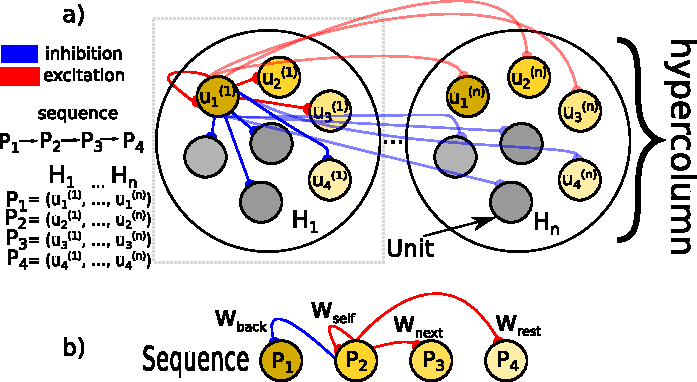
\includegraphics[scale=1.0]{diagram.pdf}
\caption{Schematic of the network structure. Units are organized in hypercolumns of which we show two H1 and H2. At each point in time only one unit is active on each of the hypercolumns.  Patterns are collections of the units that are activated in each of the hypercolumns. Pattern A for example is the activation of unit 1 in the two hypercolumns $A=(1, 1)$. We depict the stereotypical network connectivity by showing all the units that emanate from the first unit in the first hypercolumn H1. The unit connects in excitatory fashion to the proximate units on the sequence (connections from 1 to 2 and 3) but it connects in an inhibitory fashion to the units that are farther away on the sequence or not in the sequence at all (connections from 1 to the gray units or to 4).  }
\label{fig:networks_scheme}
\end{figure}


\begin{align}
\tau_s \dfrac{ds_i}{dt} &= g_{beta}\beta_i + \sum_{j} w_{ij} o_j  - g_a a_i - s_i  + \xi(t) \label{eq:simple_bcpnn} \\ 
o_i &=  \delta_{i, argmax(s)} \label{eq:simple_bcpnn_max} \\ 
\tau_a \dfrac{da_i}{dt} &= o_i - a_i \label{eq:simple_bcpnn_adaptation}
\end{align}


\subsection{The system can recall sequences}

\begin{figure}[H]
\centering
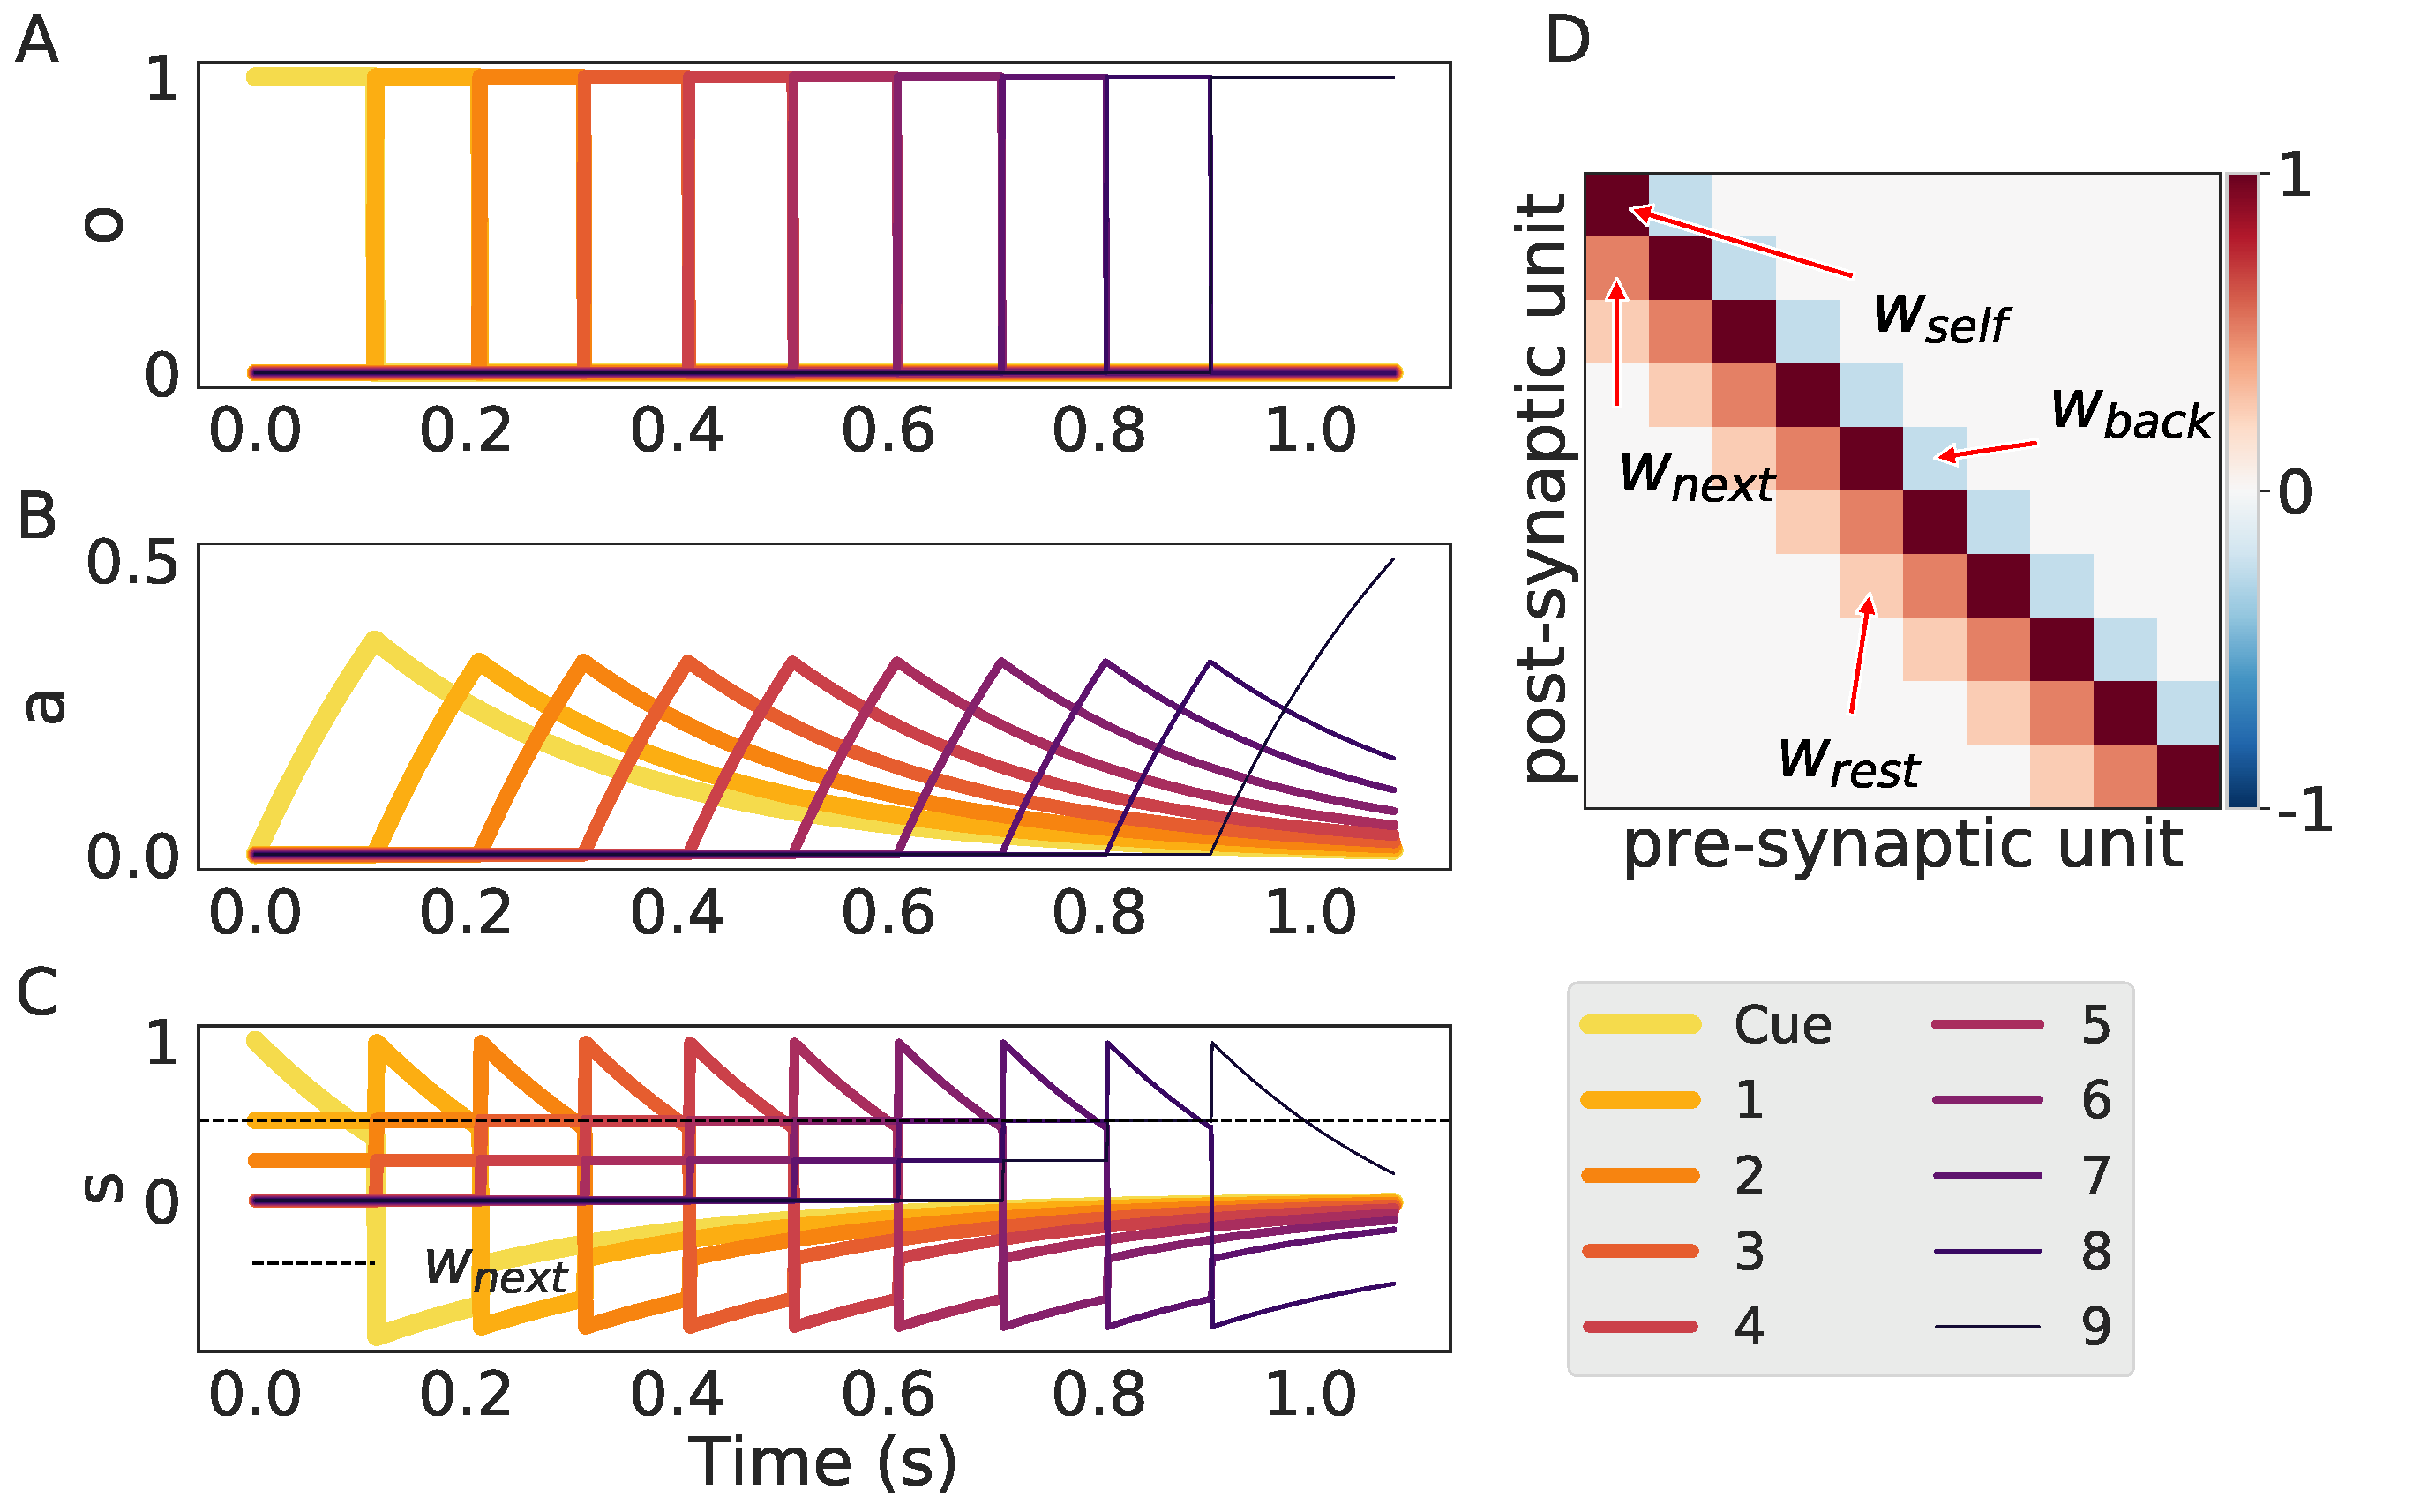
\includegraphics[scale=0.25]{simple_bcpnn_recall.pdf}
\caption{An instance of recall in the neural network. a) Unit activity starting with the cue. b) the time course of the adaptation for each unit. c) the self-excitatory current minus the adaptation current, note that this quantity crossing the value of $w_{next}$ (depicted here with a dotted line) marks the transition point from one unit to the next. d) The connectivity matrix where we have included pointers to the most important quantities $w_{self}$ for the self-excitatory weight, $w_{next}$ for the inhibitory connection to the next element, $w_{rest}$ for the biggest connection in the column after $w_{next}$ and finally $w_{back}$ for the connection to the last unit was active on the sequence.}
\label{fig:recall}
\end{figure}

\subsubsection{Analytical solution}
We can solve the deterministic equations analytical with the method of undetermined coefficients. There are two conditions, the unit that is active, and the unit that is not. 


\begin{align*} 
s(t) &= I_{fix} - g_a\left(\frac{C_{charge}}{1 - r} \right) e^{-\frac{t}{\tau_a}} + \left(s_0 - I_{fix} + g_a \left( \frac{C_{charge}}{1 - r}\right)\right)e^{-\frac{t}{\tau_s}} \\
s(t) &= \beta + w - g_a + g_a \left(\frac{1 - a_0}{1 - r}\right) e^{-\frac{t}{\tau_a}} + \left(s_0 - \beta - w + g_a - g_a \frac{1 - a_0}{1 - r}\right) e^{-\frac{t}{\tau_s}}  \\ 
s(t) &= \beta + w - g_a \left( \frac{a_0}{1 - r} \right) e^{-\frac{t}{\tau_a}} + \left(s_0 - \beta  - w  + g_a \left( \frac{a_0}{1 - r} \right) \right) e^{-\frac{t}{\tau_s}} 
\end{align*}

Where $r=\frac{\tau_s}{\tau_a}$ and $C_{charge}=a_0$ for the non-active case and $C_{charge} = a_0 - 1$ for the active case. Same for $I_{fix}=\beta + w$ for the non-active case and $I_{fix} = \beta + w - g_a$ for the active case. 

\subsection{Persistent time}

\begin{align*}
\frac{T_{ij}}{\tau_a} = \log \left(\frac{1}{1 - B_{ij}} \right) + \log \left( \frac{1}{1 - r} \right) + \log \bigg( a_i(0) + (1 - a_j(0)) \bigg) 
\end{align*}

The second term is of the order of $\tau_s$ usually and the third term accounts for memory effects on the adaptation.

Where $B_{ij} = \frac{w_{jj} - w_{ij} + \beta_j - \beta_i}{g_j}$ is a measure of inertia or inverse of speed. The close to one it is, the longer the transition takes. Also, we see that $B_{ij}$ needs to be bigger than 0 for the transition to occur, from there we can derive the criteria that $g_j > \delta w + \delta \beta$. We also introduced the short hand $f_i = \frac{1}{1 - r_i}$ which is always bigger than 1 for this system and it represents delay effects introduced due to the capacitive nature of the unit.  We see that the presence of adaptive current in the unit that is active hastens the transition ($a_j(0) > 0$  makes $T_{ij}$ smaller by reducing the second term inside the second logarithm). On the other hand, the presence of adaptive current on the next unit ($a_i(0) > 0$) in the sequence slows the process by increasing the first term in the second logarithm. 


\begin{figure}[H]
\centering
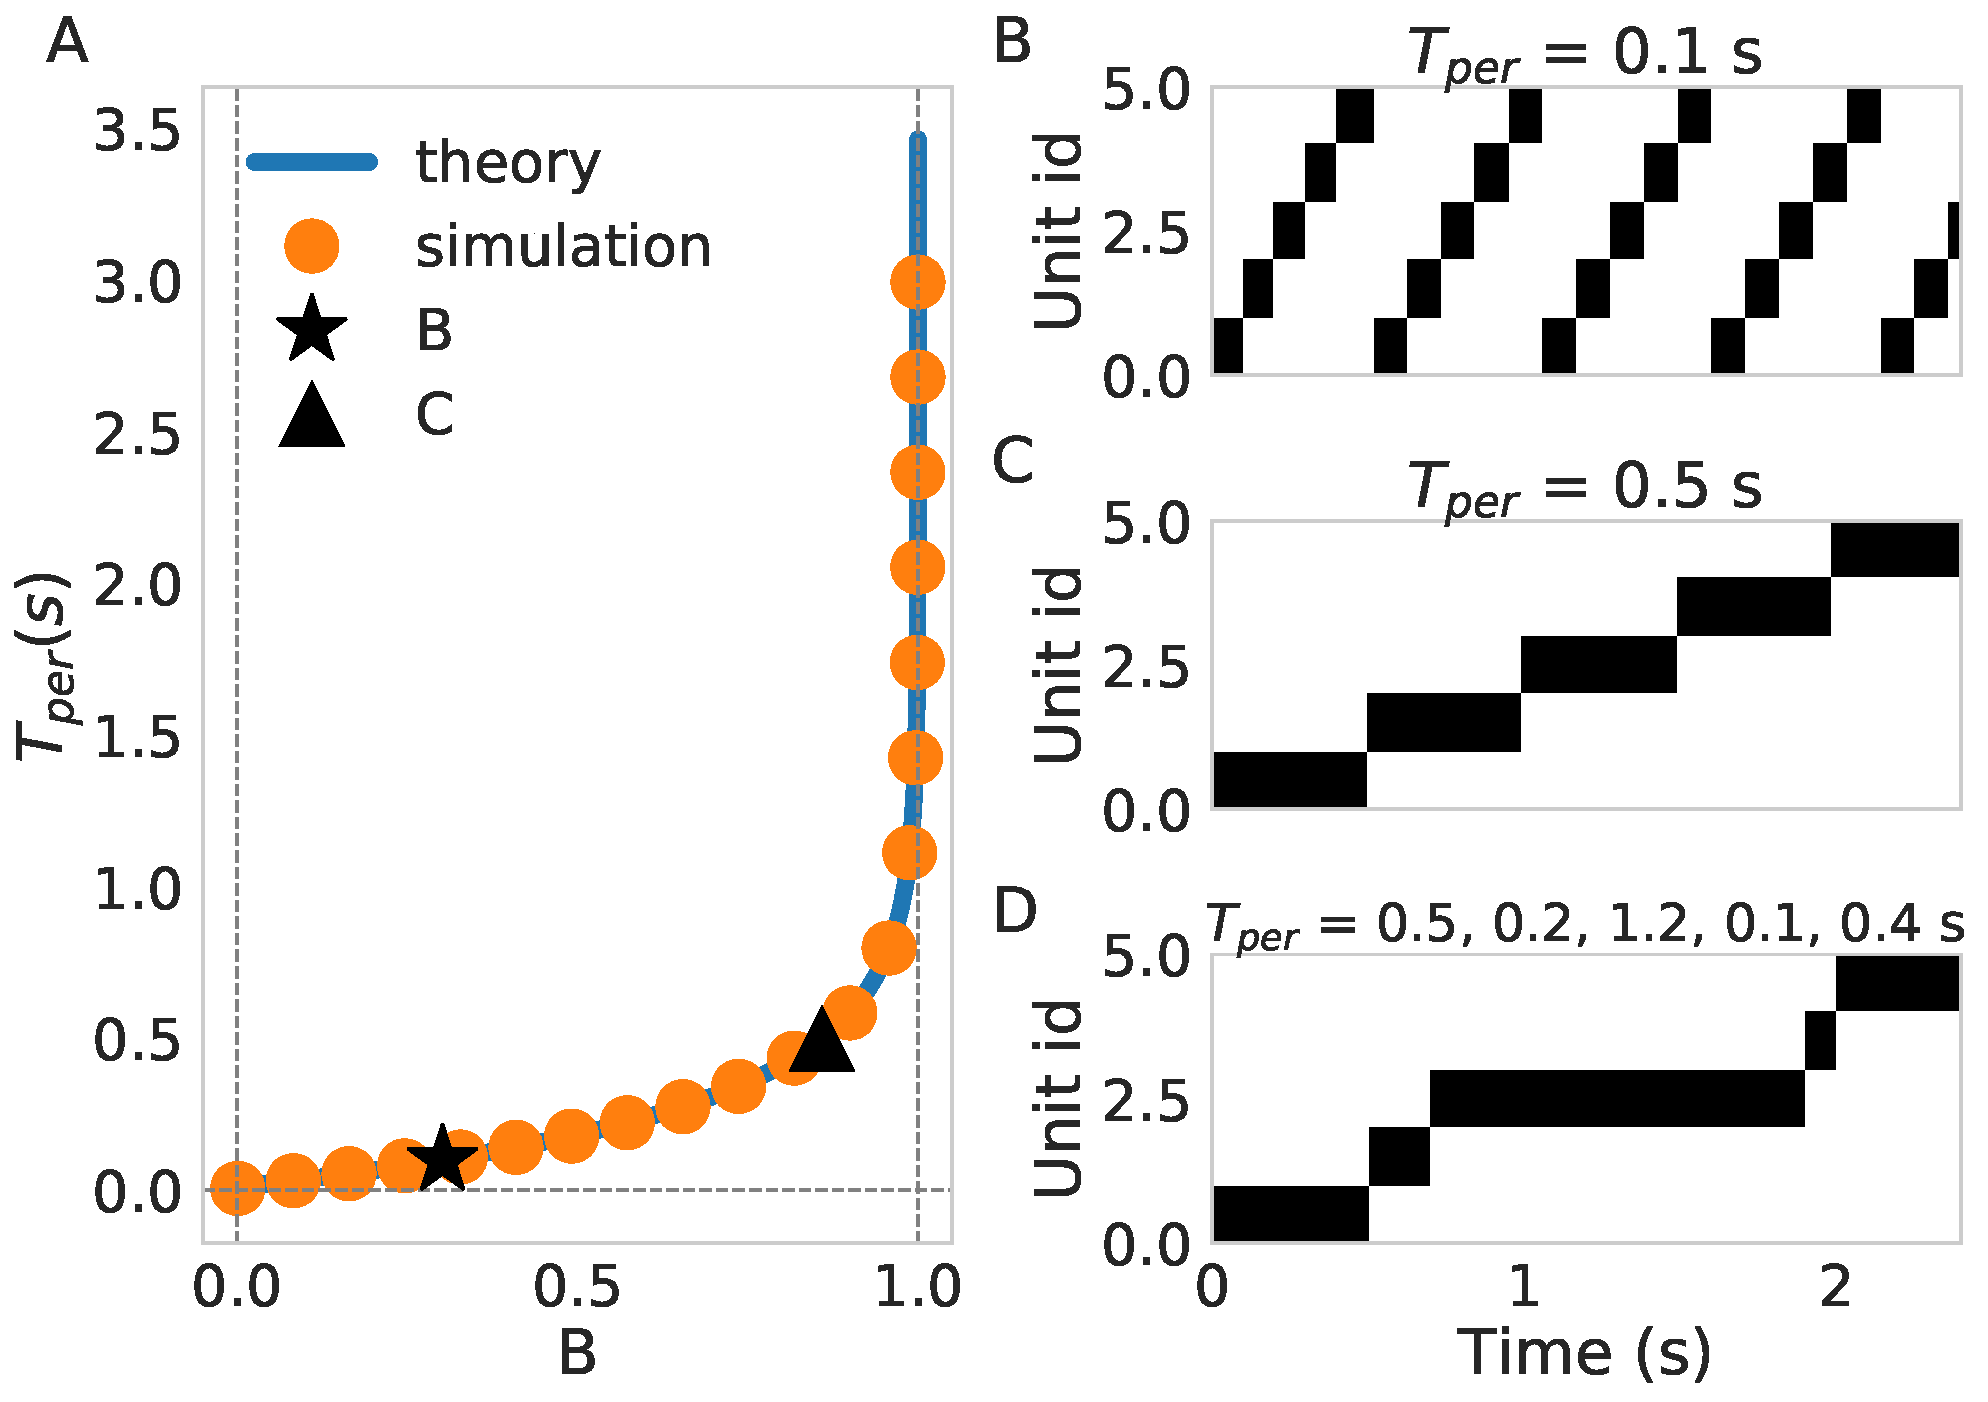
\includegraphics[scale=0.30]{persistent_times.pdf}
\caption{A characterization of persistent times. a) we show here that by controlling the parameter B between 0 and 1 we can control the persistent time of the system. To the right we show two examples of encoding first on b) there is an example of a sequence with small persistent time and  in c) another example with longer persistent time.}
\label{fig:per_time}
\end{figure}

\subsection{Learning}
\begin{figure}[H]
\centering
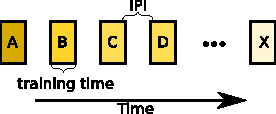
\includegraphics[scale=1.40]{protocol.pdf}
\caption{The training protocol. We show here the basic scheme of the training protocol used in the system. We pass the patterns in close succession to each other and they are characterised first by their training time, that is, how long is the system exposed (units are clamped) to the pattern and second by their inter pulse interval (IPI) which is the time in between the unit's activation. Note that this need not to be equal for each pattern.}
\label{fig:training_protocol}
\end{figure}


\begin{figure}[H]
\centering
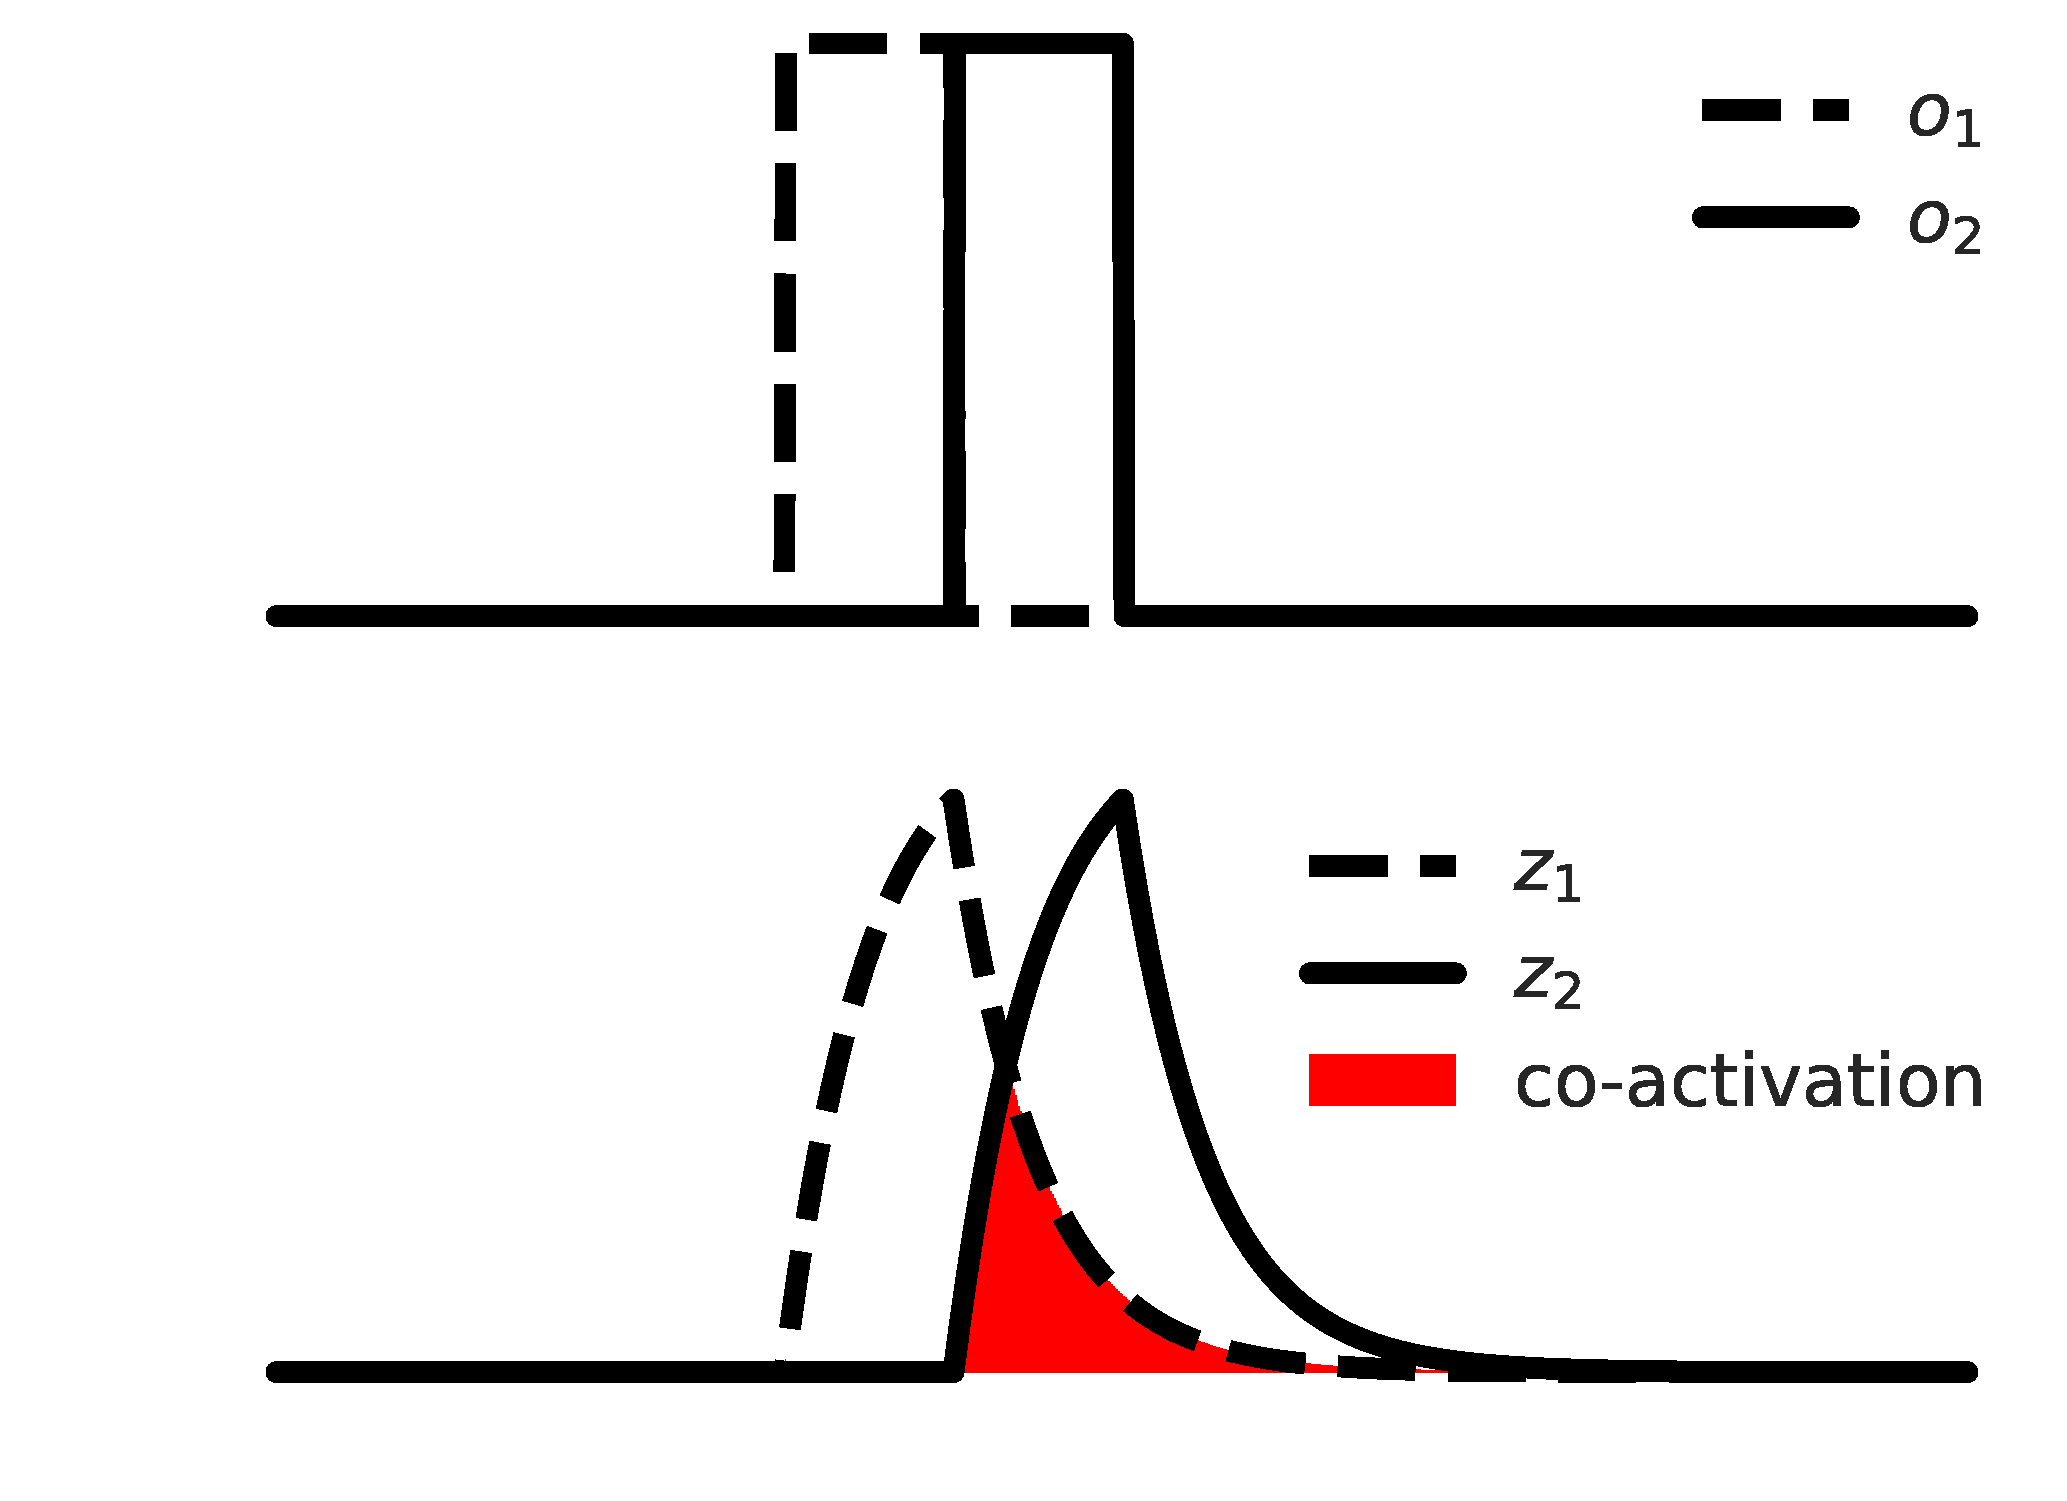
\includegraphics[scale=0.30]{traces_example.pdf}
\caption{Learning by traces. The system weights the intersection of two traces (co-activation) against the base activation rate of each unit to determine the magnitude of the weight between two units. }
\label{fig:traces_example}
\end{figure}

\begin{figure}[H]
\centering
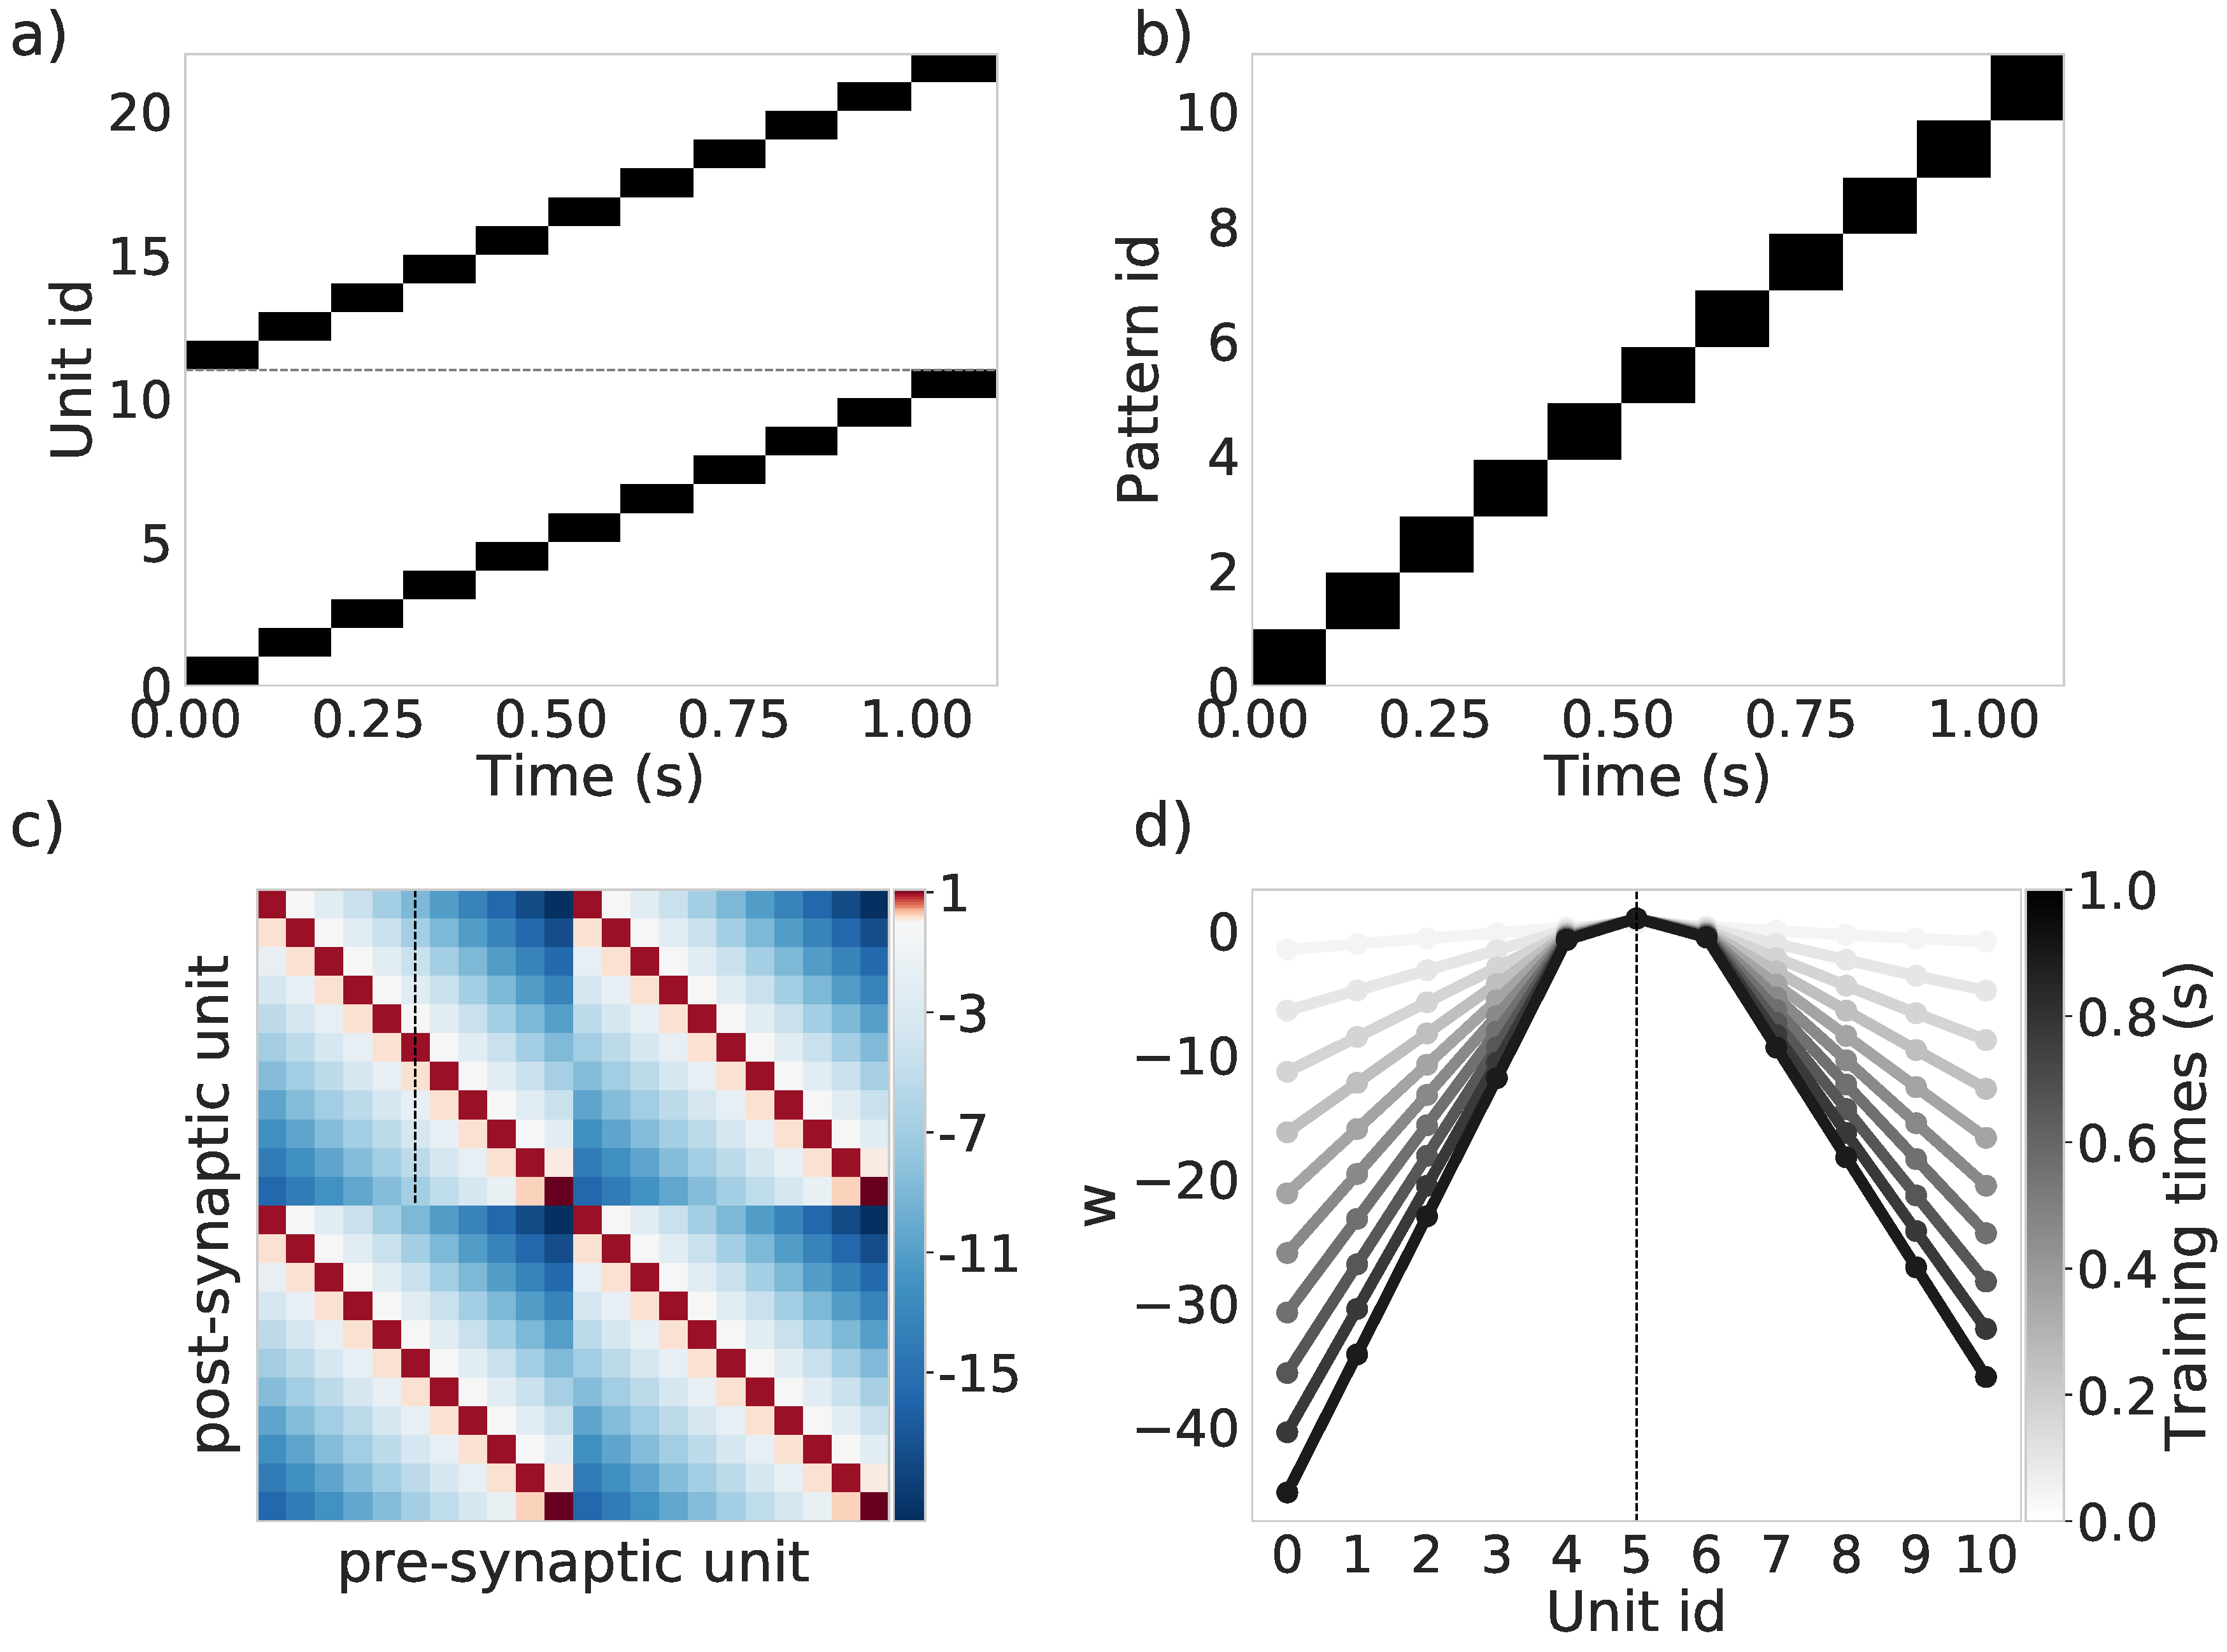
\includegraphics[scale=0.20]{recall_example.pdf}
\caption{An example of recall with 10 minicolumns and 2 hypercolumns, $\tau_{z_{pre}} = \tau_{z_{post}}=25 \, ms$, training times $=100 \, ms$ and $IPI = \, 0 $. We show in a) how the recall phase in a system with learned connectivity looks like. b) We show how close (1 - cosine distance) the instant activity of the network is to the stored pattern at every point in time. c) The connectivity matrix for this particular example, note that the modularity is an outcome of the hypercolumn organization. We show the profile of connections of the dashed line on d) for a variety of training times. Darker lines represent longer training times. }
\label{fig:recall_example}
\end{figure}

\begin{figure}[H]
\centering
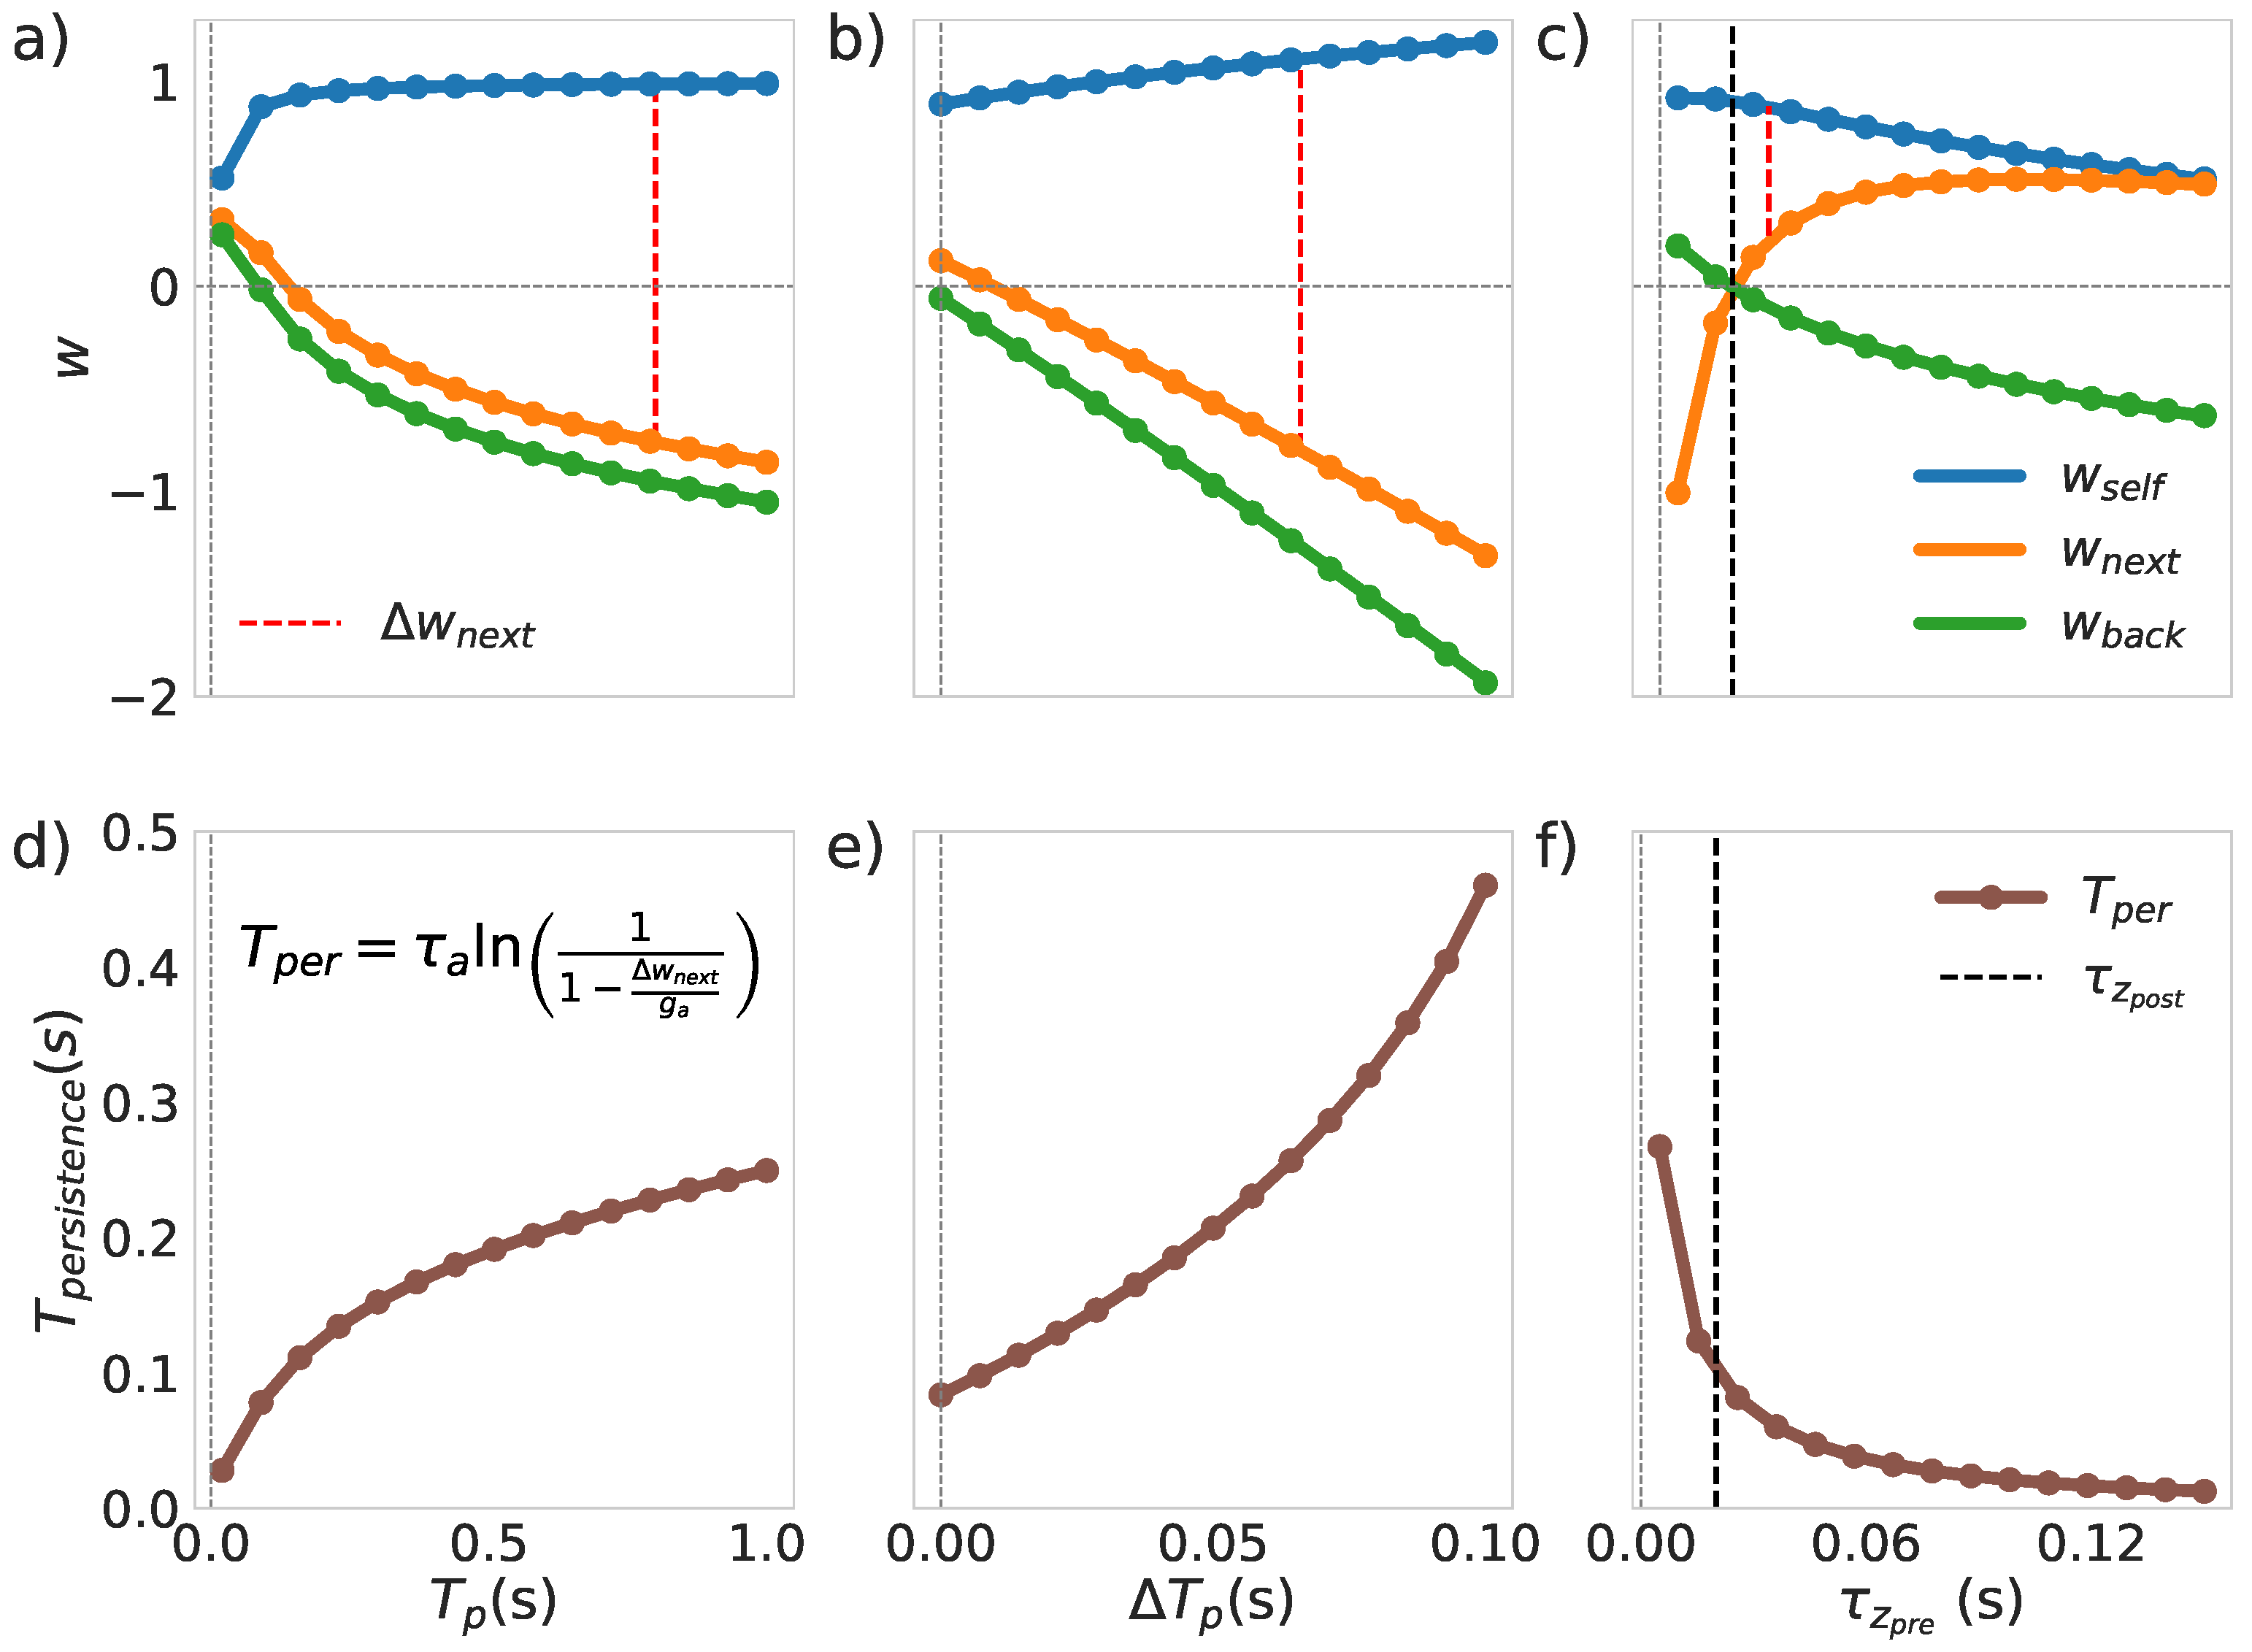
\includegraphics[scale=0.20]{training.pdf}
\caption{Characterization of the connectivity as a function of the training protocol. Here we show how the $w_{self}$, $w_{next}$, $w_{back}$ depend on the training protocol parameters. We also show how $B$, $T_{persistence}$ $\Delta w_{next} = w_{self} - w_{next}$ to directly illustrate the effect of training on the persistent time of the attractors. When the parameters themselves are not subjected to variation their values are training time = $100 \, ms$, IPI $= 0 \, ms$, $\tau_{z_{pre}}  = 25 \, ms$, $\tau_{z_{post}}= \, 20 ms$ for all the units In the following explanation everything that we say about $w_{next}$ can be applied to $w_{back}$ as they are generated with the same process but with a different time constant on their filters. a) we observe that as the training time increases the value of $w_{self}$ quickly stabilizes but the value of $w_{next}$ becomes smaller. This can be explained by the fact that while the self co-activation remains constant with respect to the complete training protocol (stabilizing $w_{self}$) the co-activation between units becomes a smaller portion of the whole training protocol (making $w_{next}$ smaller). This is also reflected on d) where we see that $\Delta w_{next}$ increases slower with bigger training times and so do in consequence $B$ and $T_{persistence}$.  We see on b) that $w_{self}$ keeps increasing while $w_{next}$ is decreasing with longer IPIs. The longer IPIs bring about an overall longer training protocol which makes the self co-activation more meaningful and $w_{self}$ bigger. $w_{next}$, on the other hand, naturally decreases as a longer IPI makes the co-activation between the units smaller as their activations are father from each other in time. e) we can observe the effect of this dynamic for $\Delta w_{next}$ and $B$ which grow linearly and cause $T_{persistence}$ to increase logarithmicaly with longer IPIs. In c) we can appreciate that the effect of increasing $\tau_{z_{pre}}$ is to make the time coincidence of units in time less important. This is reflected by the fact that $w_{self}$ which reflects the self-activation becomes smaller and that the $w_{next}$ becomes bigger. Note here that when $\tau_{z_{pre}}$ becomes bigger than $\tau_{z_{post}}$ (marked with a dashed red line) coincides with $w_{next}$ becoming bigger than $w_{back}$ as we should expect. As we are able to observe in f) $\Delta w_{next}$ becomes almost zero for big values of $\tau_{z_{pre}}$ which makes encoding patterns difficult on this regime of parameters. }
\label{fig:training}
\end{figure}

\subsection{Noise}

\begin{figure}[H]
\centering
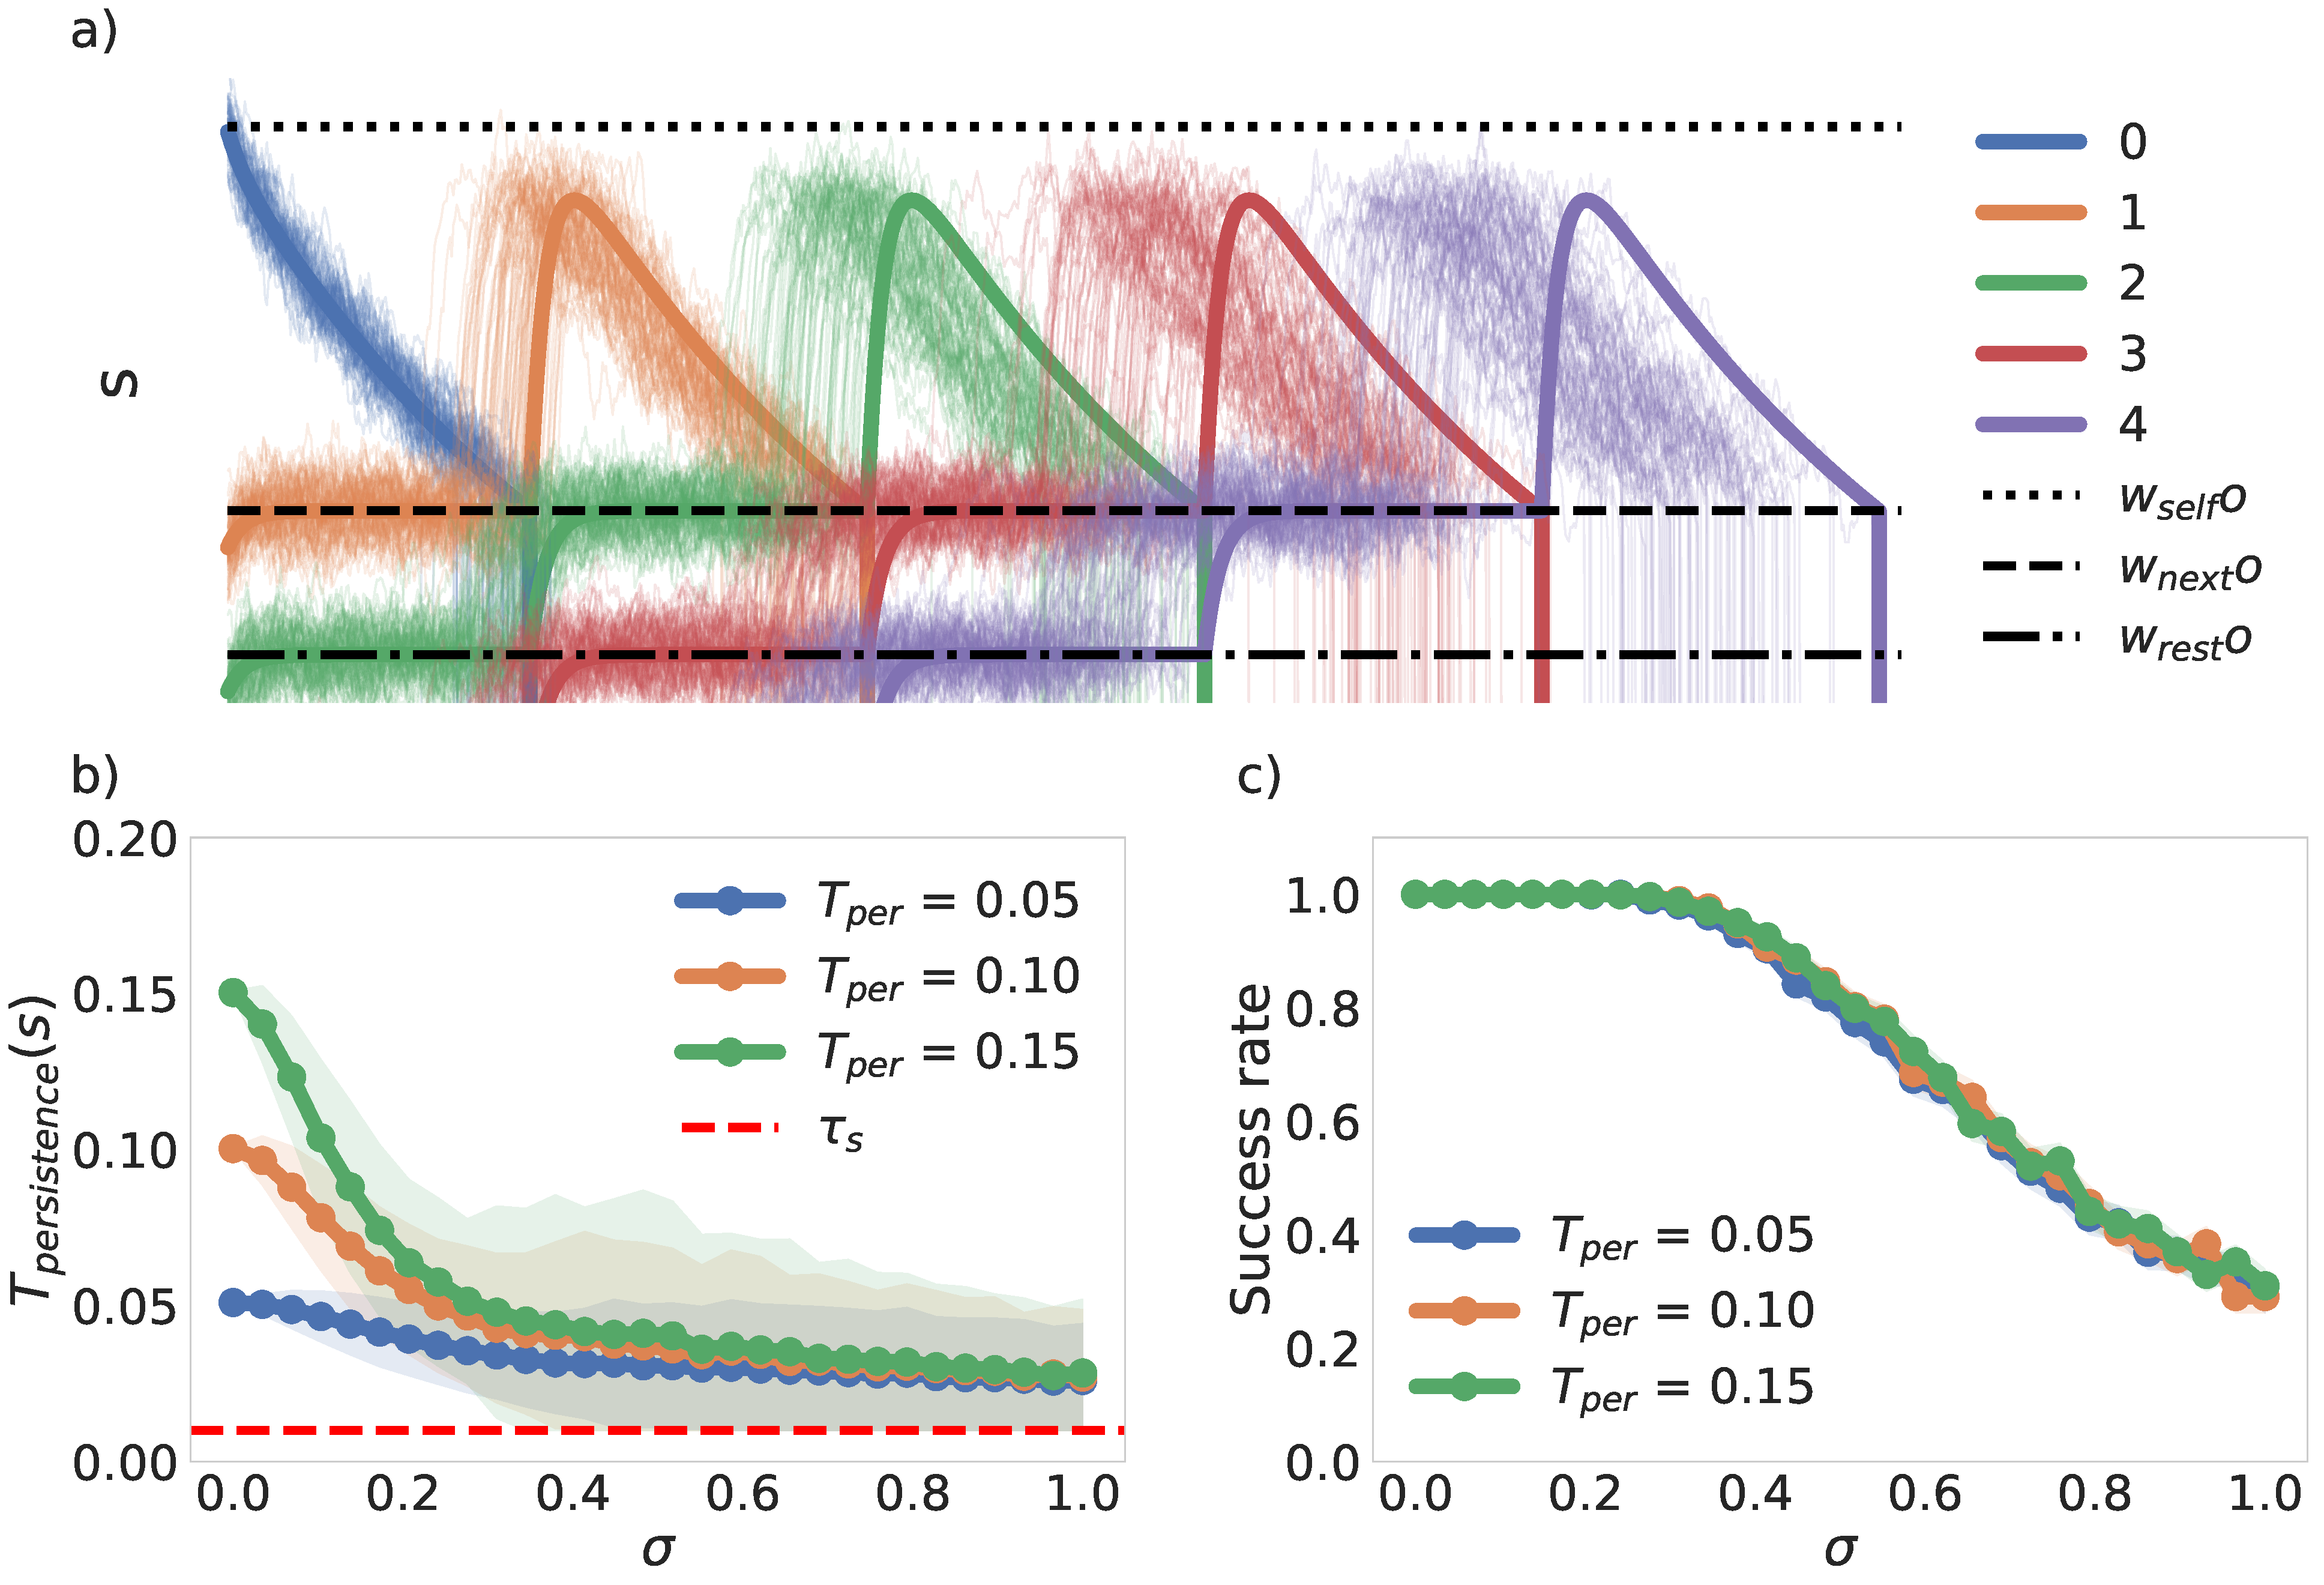
\includegraphics[scale=0.17]{noise_diagram.pdf}
\caption{Effects of noise in trajectories and persistent time. a) we show here an example of noisy trajectories as they evolve in time. The solid lines indicate the deterministic trajectories the system would follow in zero noise case. In dotted, jagged and dashed lines we depict the important landmark of connectivity $w_{self}$, $w_{next}$ and $w_{rest}$ respectively. We can notice that in the noisy case the units make the transition to the next unit faster that they would have done in the deterministic case. This is show bellow were even if the success vs noise profile is not affected by variations $T_{persistence}$  as we can appreciate in b) we can observe in c) that mean $T_{persistence}$ quickly decays with noise.}
\label{fig:noise_scheme}
\end{figure}

\begin{figure}[H]
\centering
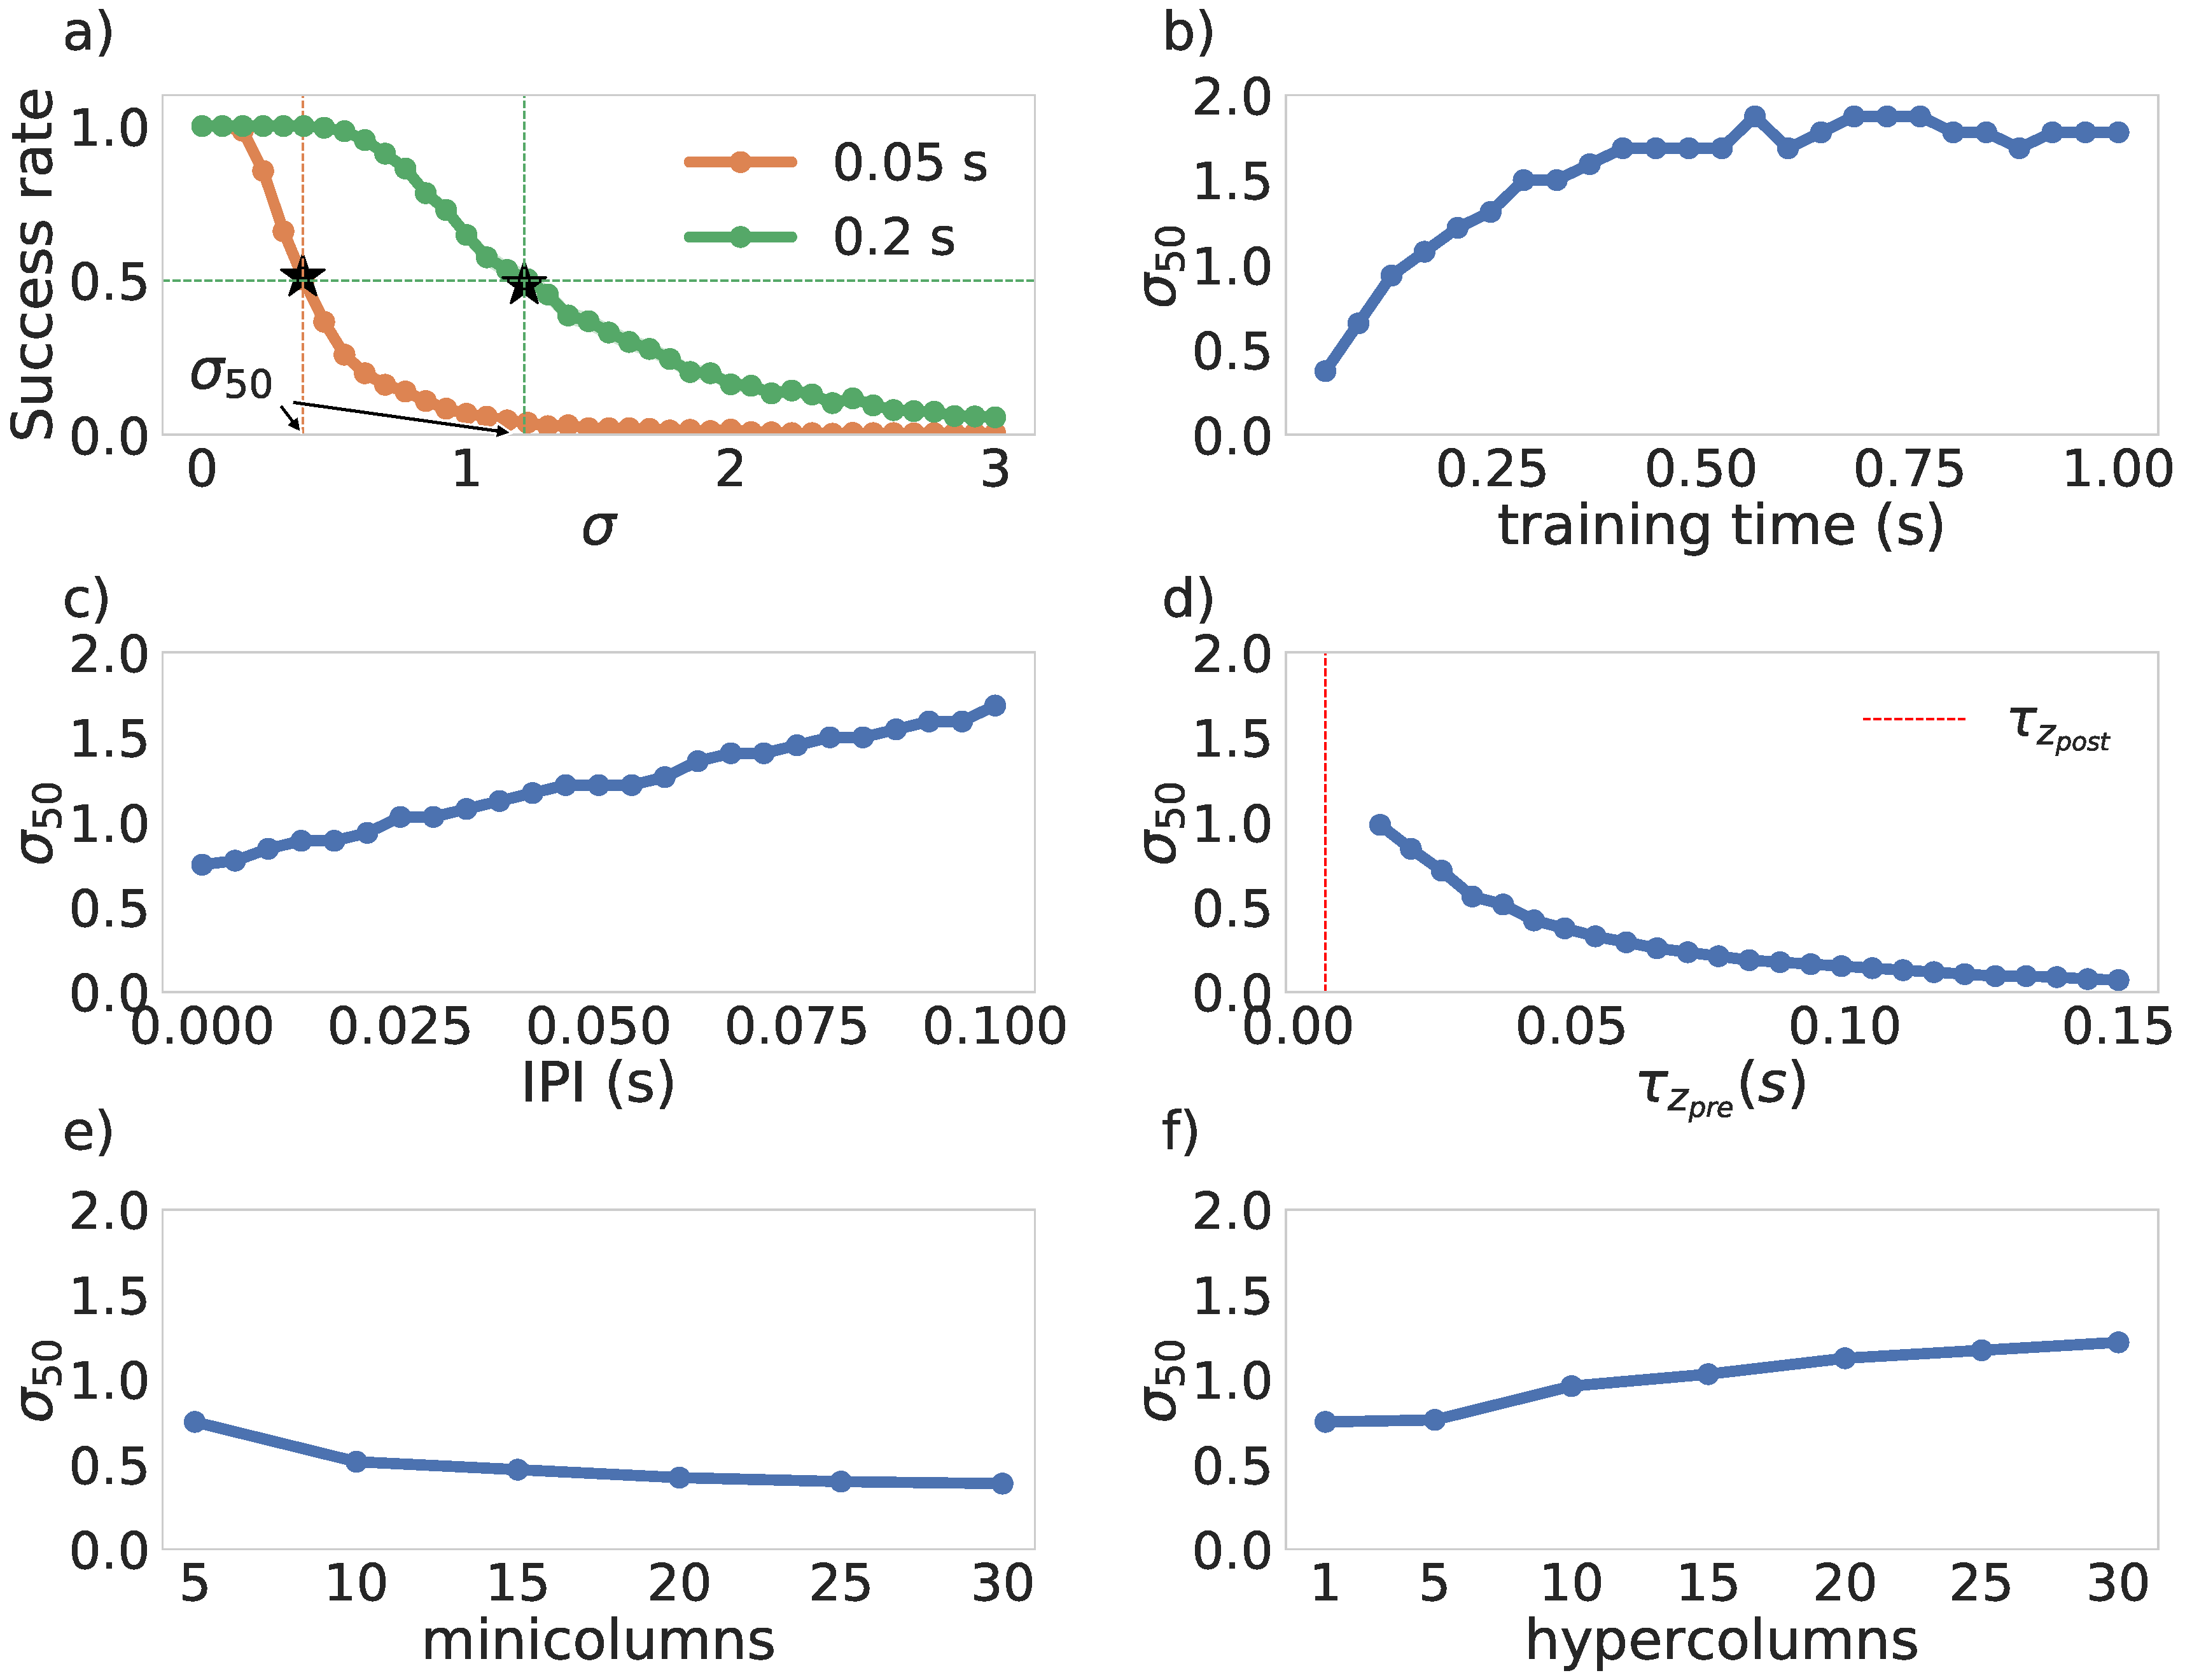
\includegraphics[scale=0.20]{noise_robustness.pdf}
\caption{We characterized  how robust the networks that we train are to noise in their recall phases. To do this we calculated how likely is the network to retrieved a cue recalled sequence succesfully for different levels of noise. We use the following parameters for all the training except when the parameter itself was varied: training time $= 100 \: ms$, IPI $= 0 \: ms$, $\tau_{z_{pre}} = 25 \: ms$, $\tau_{z_{post}} = 100 \: ms$ minicolumns $=5$, hypercolumns$=1$. a) Two examples of the success vs recall profile for two neural networks ($50 \: ms$ and $200 \: ms$. We also annotated in black the points at which the probability reached its half valued, we call the argument $\sigma_{50}$ and we use its dependency on the parameters as a way to quantify the variance of robustness with noise, that is, the bigger $\sigma_{50}$ is the more robust the system is to noise and vice versa. b) $\sigma_{50}$ with respect to training, we can see that the system becomes more robust the longer it sees the patterns. c) }
\label{fig:robustness}
\end{figure}


\subsection{Representations}

\begin{figure}[H]
\centering
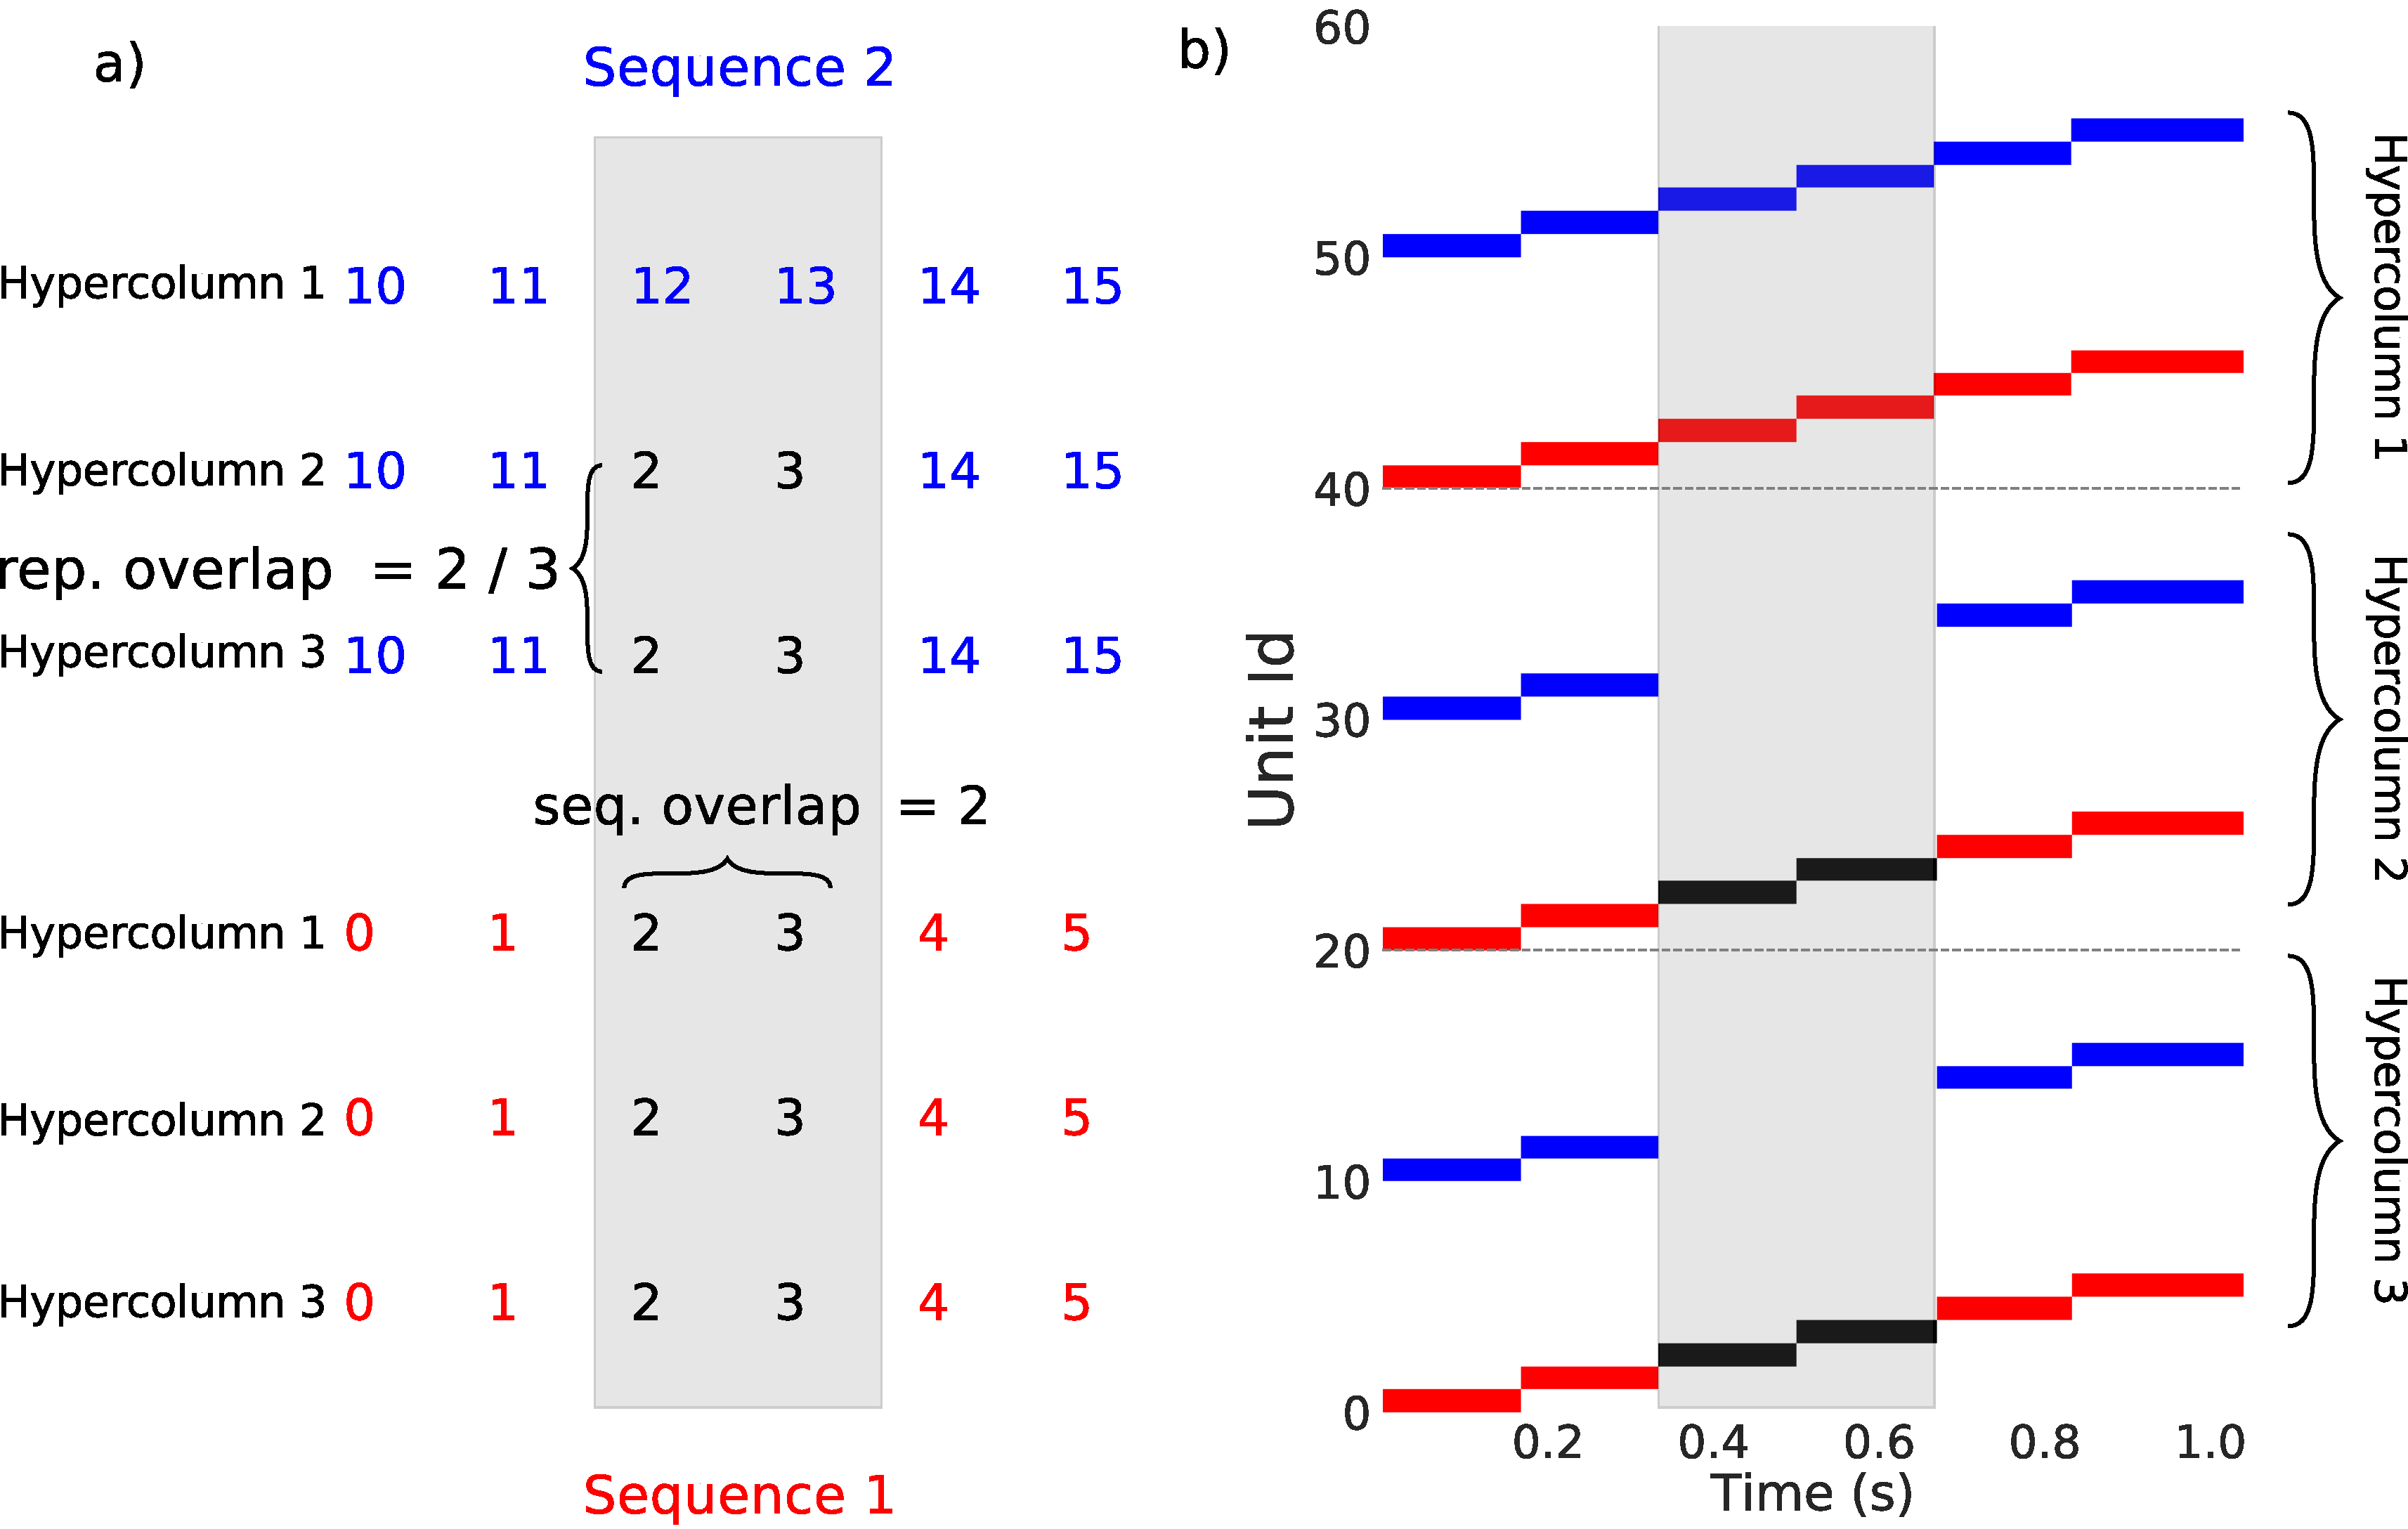
\includegraphics[scale=0.20]{rep_diagram.pdf}
\caption{Overlap diagram}
\label{fig:rep_diagram}
\end{figure}

\begin{figure}[H]
\centering
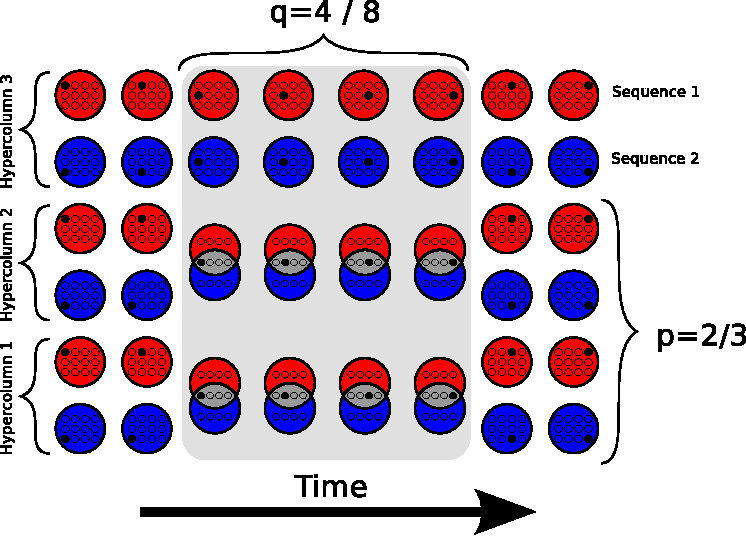
\includegraphics[scale=0.90]{overlap_diagram.pdf}
\caption{Overlap diagram}
\label{fig:representation_scheme}
\end{figure}

\begin{figure}[H]
\centering
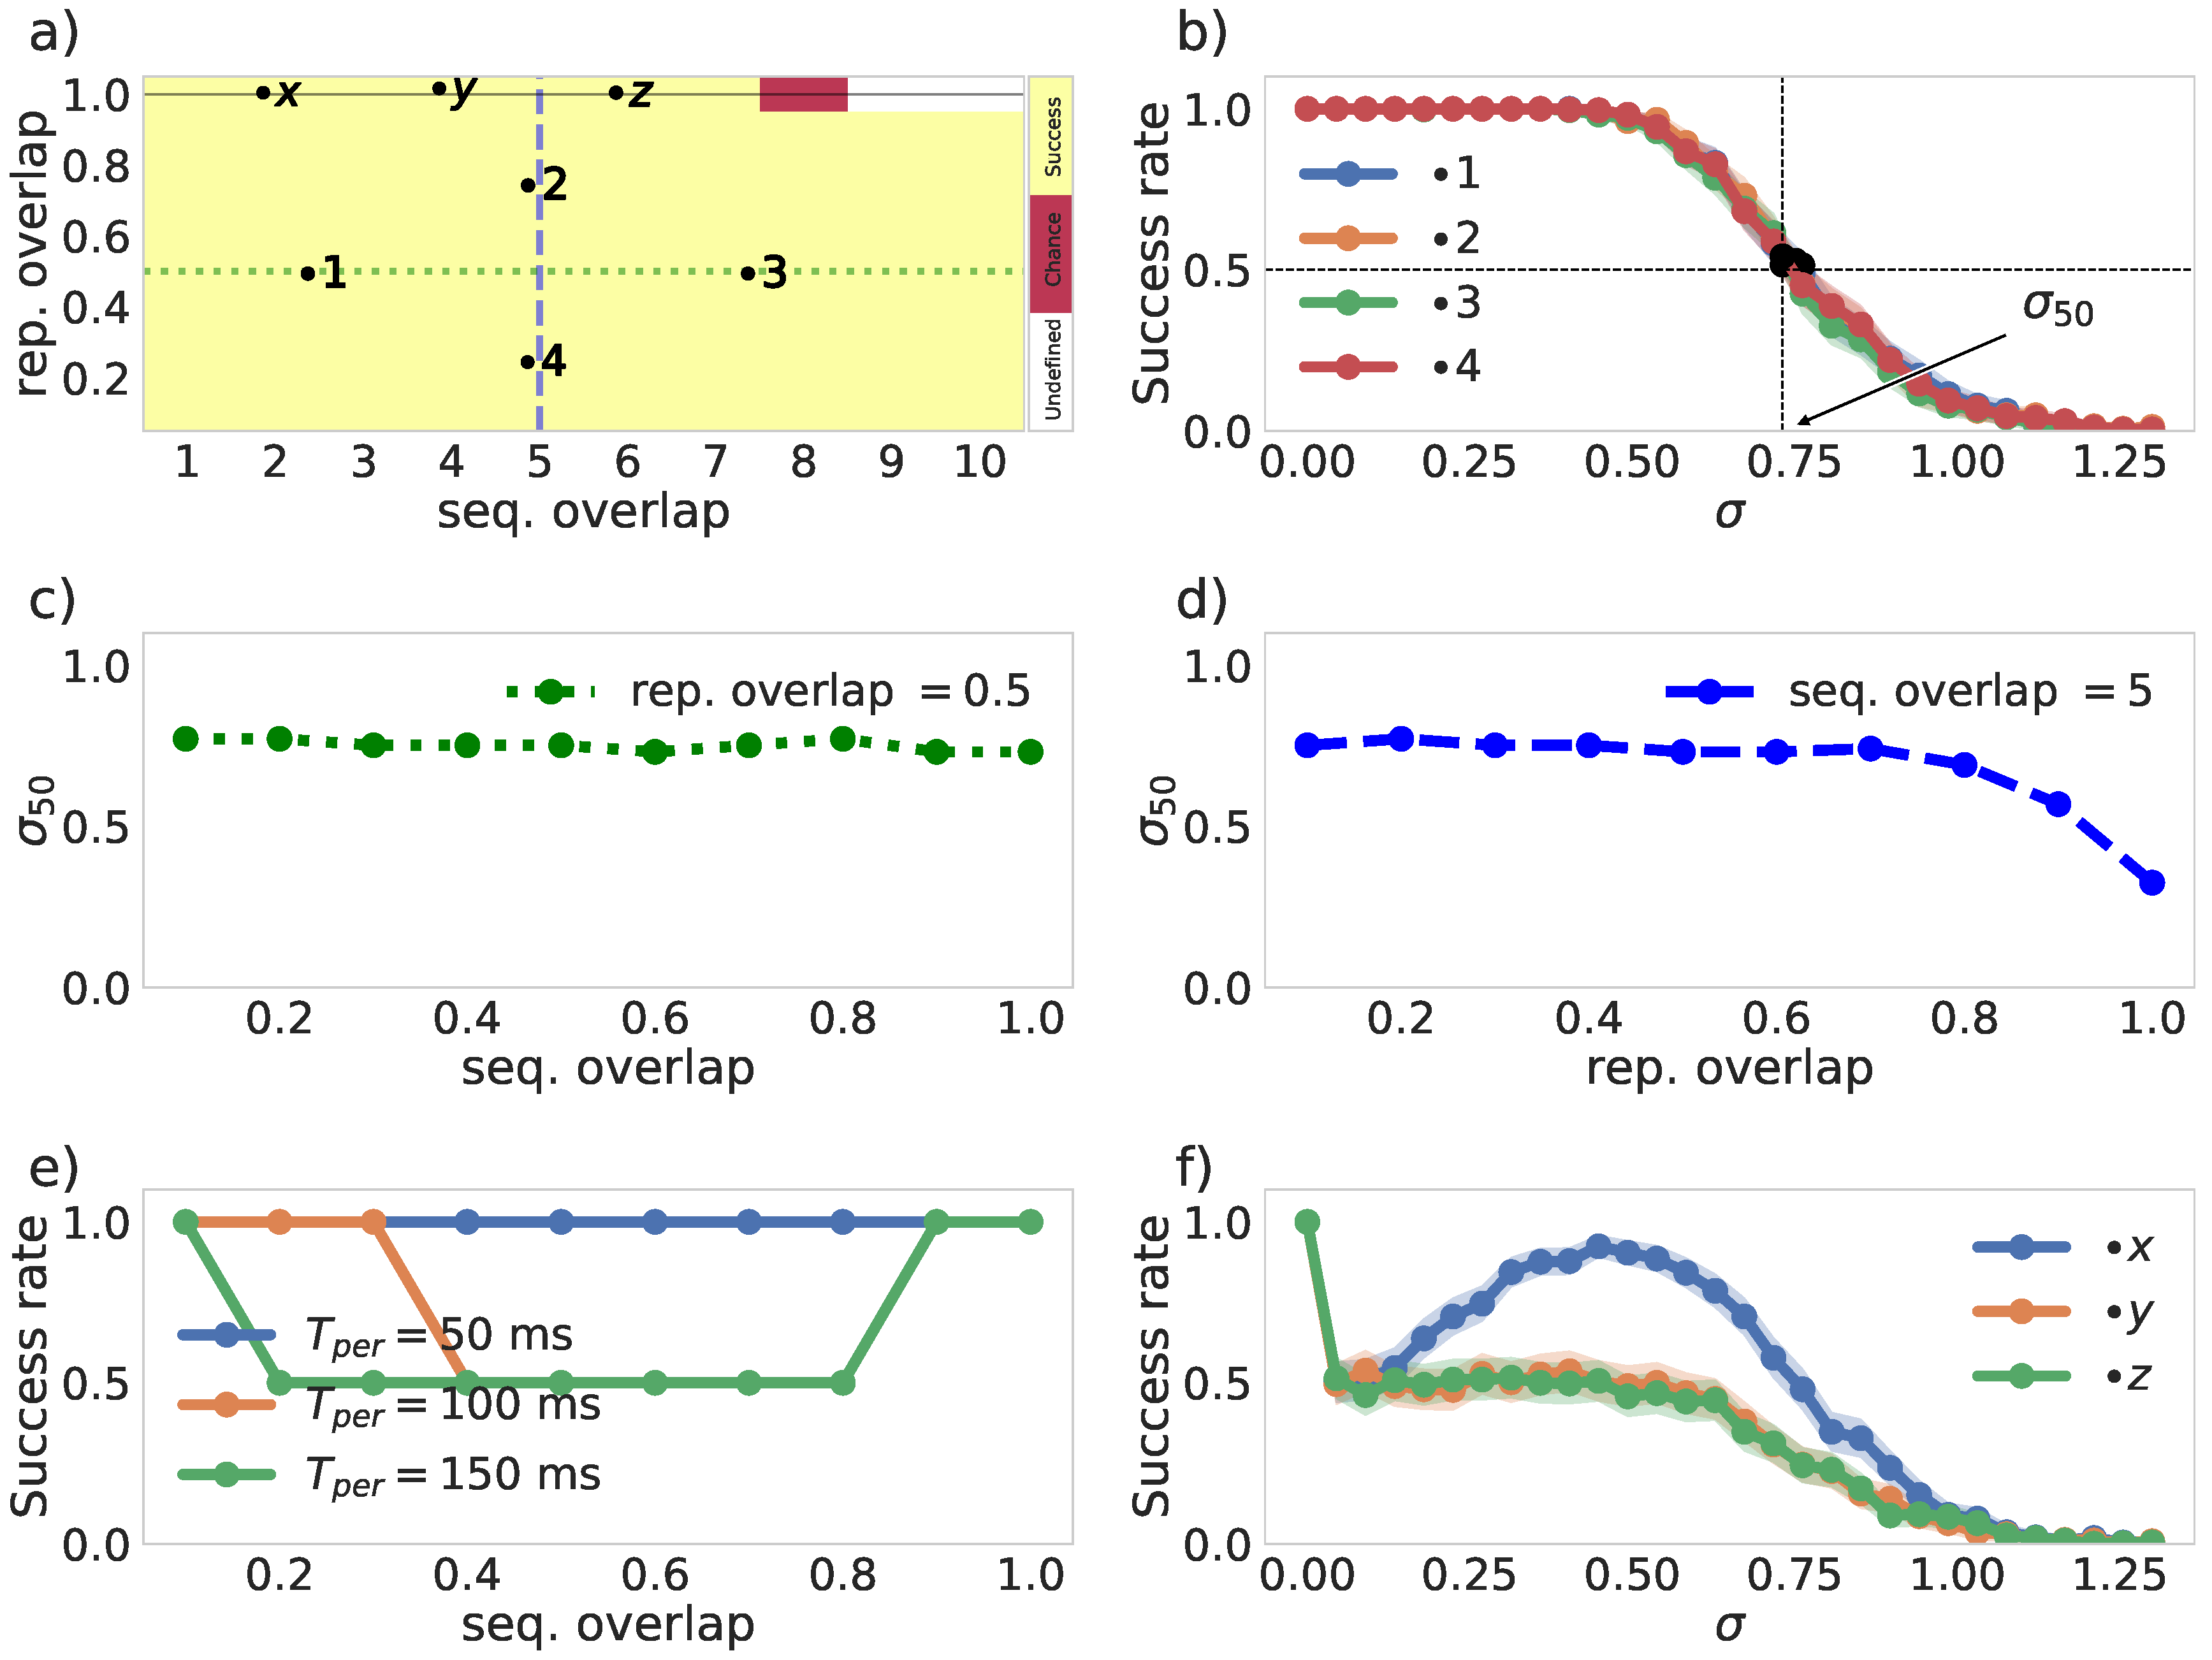
\includegraphics[scale=0.20]{representations.pdf}
\caption{A characterization of the different overlap conditions}
\label{fig:representations}
\end{figure}


\subsection{Non-homogeneous training conditions}

\begin{figure}[H]
\centering
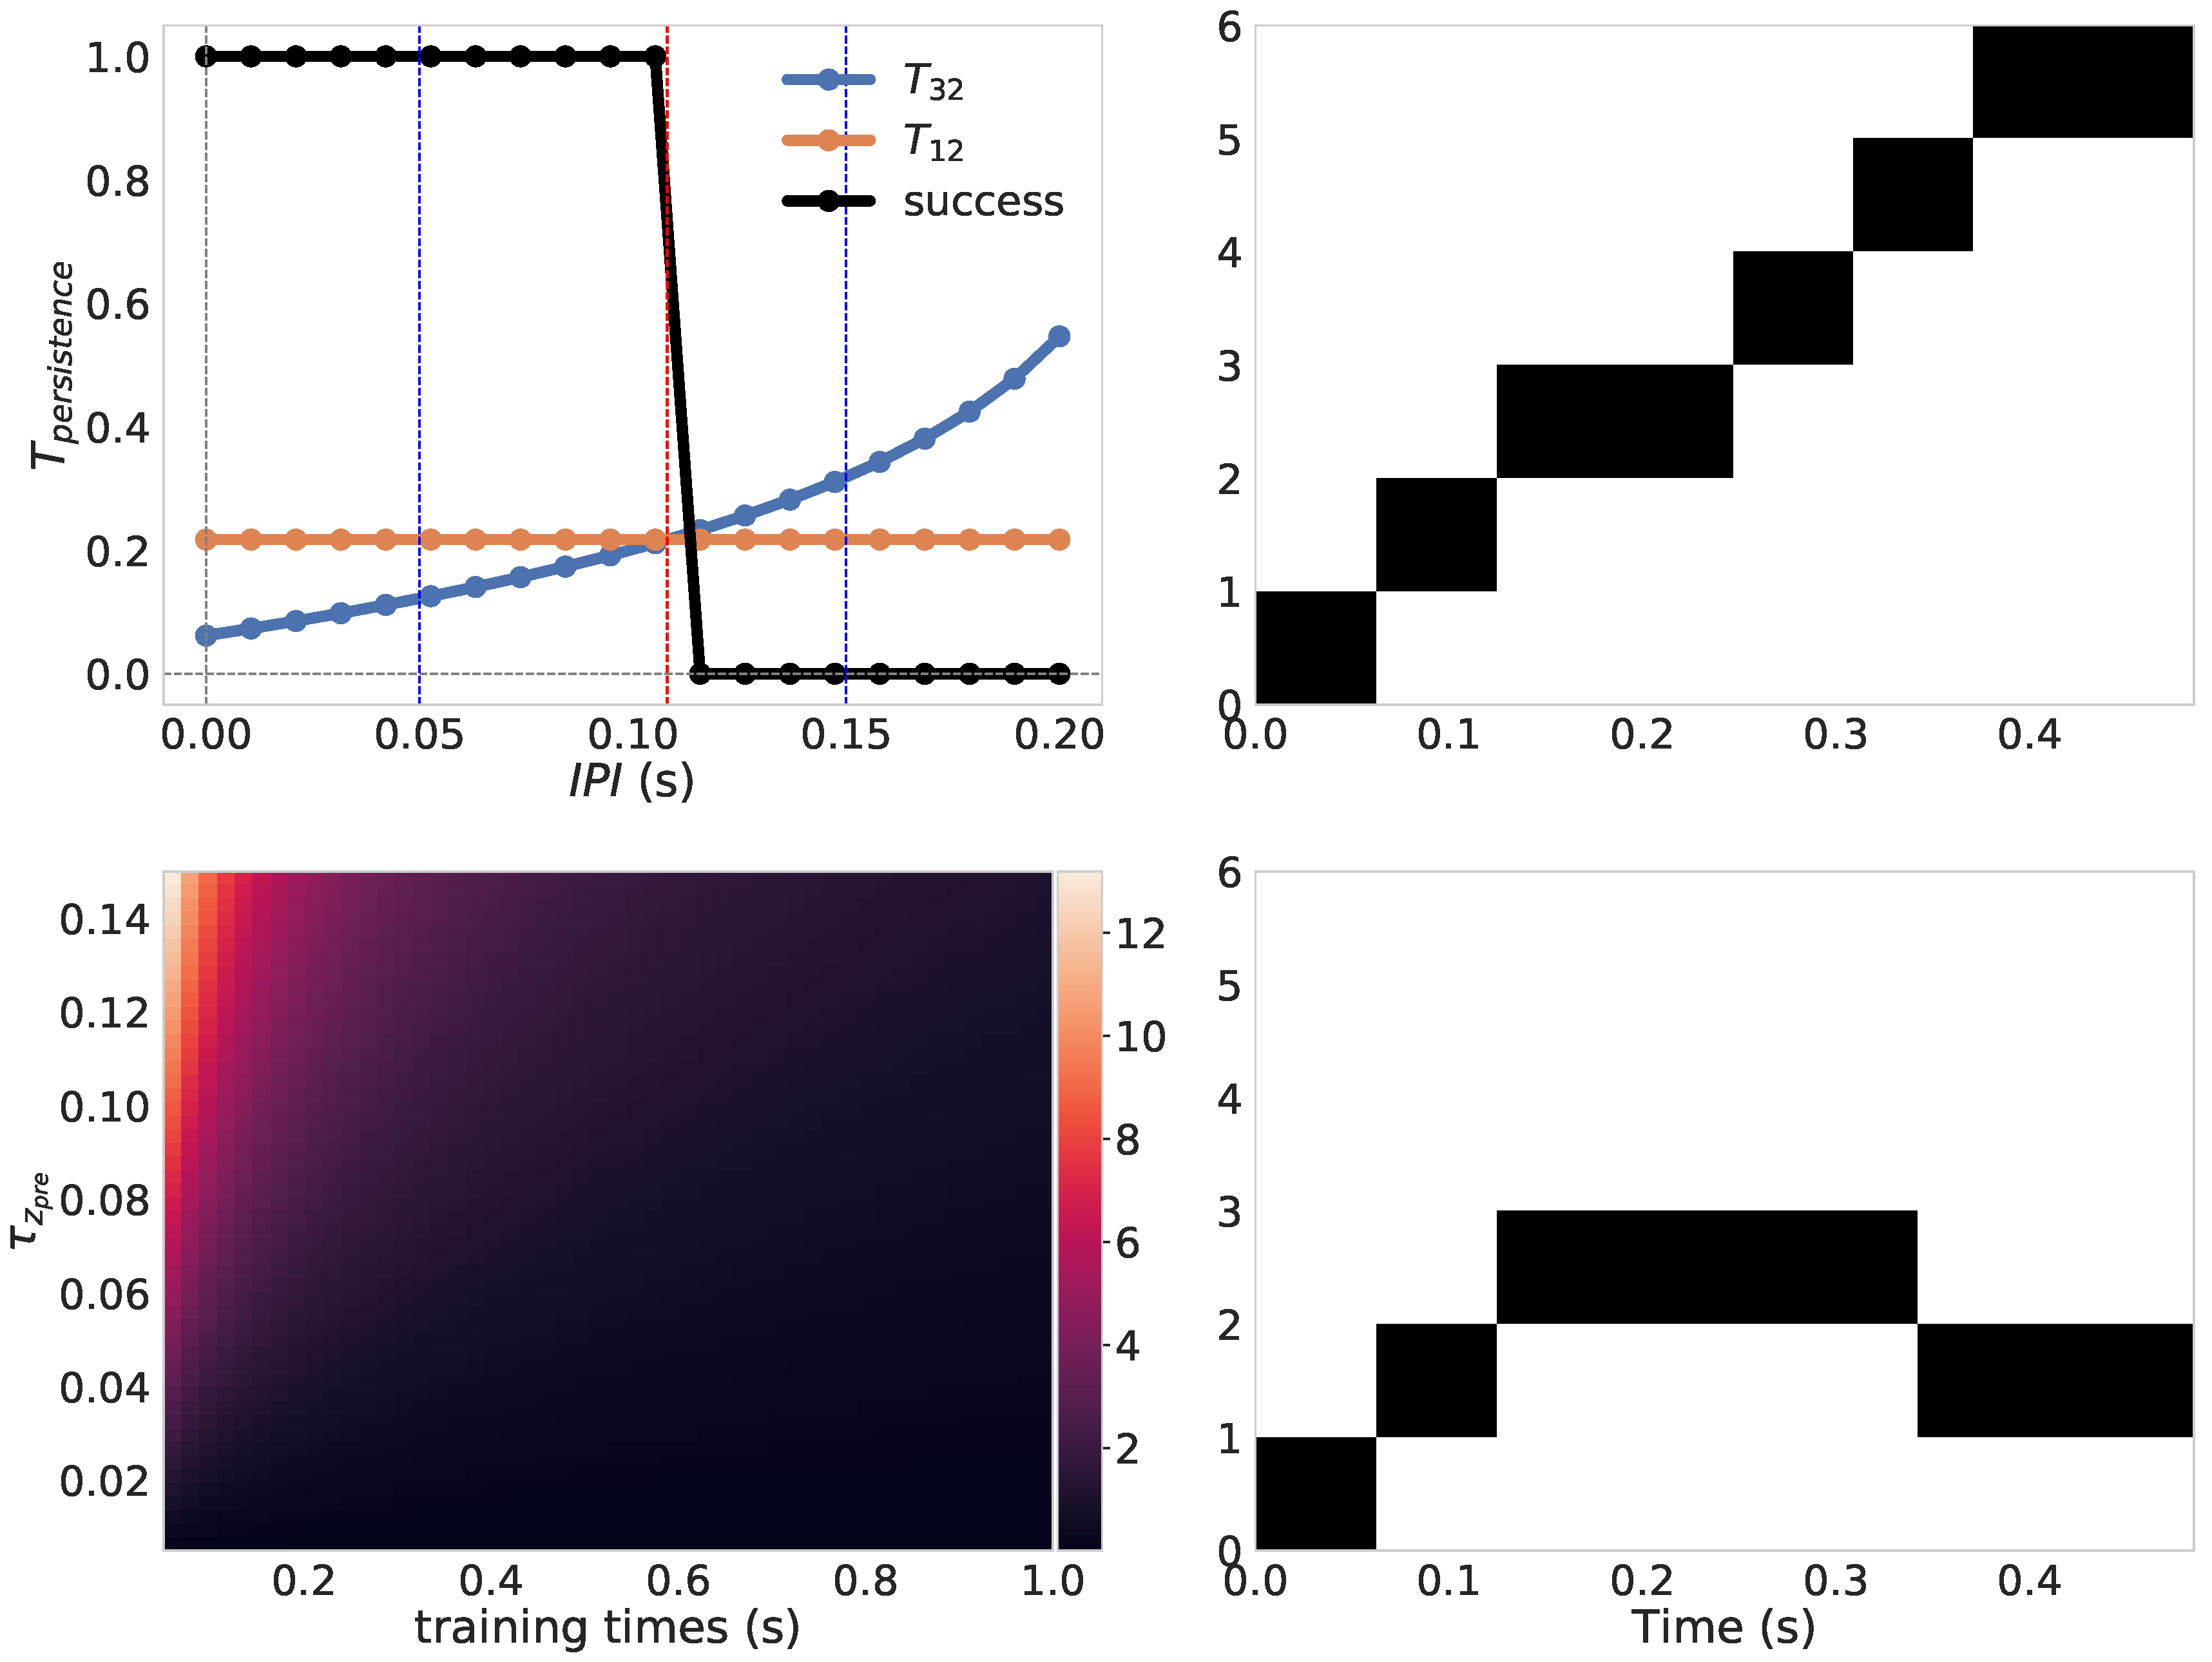
\includegraphics[scale=0.20]{ipi_non_homogenous.pdf}
\caption{A characterization of the different overlap conditions}
\label{fig:non-homo}
\end{figure}


%\bibliographystyle{unsrt}
%\bibliography{references.bib}

\end{document}